%%%%%%%% ICML 2022 LATEX SUBMISSION FILE %%%%%%%%%%%%%%%%%
\documentclass[nohyperref]{article}

\def\inchome{../include}
\def\fighome{../figures}
\def\bibhome{../bib}
\def\texhome{tex}

\usepackage{lineno,microtype}

\usepackage[colorlinks=true,linkcolor=blue,citecolor=green,urlcolor=black]{hyperref}
\usepackage{xspace}

%\usepackage{times}
%\usepackage[square,sort,comma,numbers]{natbib}
%\usepackage{natbib}
%\usepackage[outdir=./]{epstopdf}
\usepackage{graphicx,float,pgfplots,wrapfig,sidecap,lipsum}
\usepackage{tabularx}
\usepackage{booktabs}
\usepackage{paralist}
%\usepackage{algorithm}
%\usepackage[noend]{algorithmic}
% \usepackage[pass]{geometry}
\usepackage{amsfonts}
\usepackage{amsthm}
\usepackage{amsmath}
\usepackage{amssymb}
\usepackage{mathrsfs}
\usepackage{xcolor}
\definecolor{lightblue}{RGB}{240,245,255}
% https://www.overleaf.com/1596253897kwtdtqtgvgtk
\definecolor{darkblue}{RGB}{40,40,85}
\usepackage{listings}
\lstset{
    language=python,
    backgroundcolor = \color{lightblue},
    basicstyle=\scriptsize\fontfamily{SourceCodePro-TLF}\selectfont,
    breaklines=true,
    showstringspaces=false,
    keywordstyle=\color{green!25!black},
    commentstyle=\itshape\color{gray},
    numberstyle=\color{blue},
    morekeywords={var, f32, i32, layout, ti, kernel, layout, func},
    classoffset=1,
    morekeywords={kernel, bitmasked, morton, pointer},
    keywordstyle=\color{darkblue},
    classoffset=2,
    morekeywords={root, dense, dynamic, hash, Index, Indices, Vector, Matrix, Var, AssumeInRange, Parallelize, Vectorize, Cache, CacheL1, BlockDim, Atomic},
    keywordstyle=\color{green!50!black},
    classoffset=3,
    morekeywords={place},
    keywordstyle=\color{blue},
%    moredelim=**[is][\color{red}]{@}{@},
    xleftmargin=0.1cm,
    xrightmargin=0.1cm,
    frame=tlbr,
    framesep=0.1cm,
    framerule=0pt
}

\usepackage{enumerate}
\usepackage{enumitem}
%\usepackage{xcolor}
\usepackage{mathtools} 

\usepackage{tablefootnote}
\usepackage{caption}
\usepackage{subcaption}
\usepackage[normalem]{ulem}
\usepackage{psfrag}
\usepackage{tikz}
\usetikzlibrary{fit}
\usetikzlibrary{calc,shapes}
\usetikzlibrary{decorations.pathmorphing} % noisy shapes
\usetikzlibrary{fit}					% fitting shapes to coordinates
\usetikzlibrary{backgrounds}	% drawing the background after the foreground

\usepackage{bm}
\usepackage{cleveref}

\usepackage{stmaryrd}
\usepackage[utf8]{inputenc}
\usepackage[english]{babel}

\usepackage{multirow}
\usepackage{tabularx}
\usepackage{makecell} %\thread

\usepackage{graphicx,float,pgfplots,wrapfig,sidecap,lipsum}
\pgfplotsset{compat=1.16}

\usepackage{tikz}
\usetikzlibrary{calc,trees,shadows,positioning,arrows,chains,shapes.geometric,decorations.pathreplacing,decorations.pathmorphing,shapes,
matrix,shapes.symbols,patterns,intersections,fit}
\newcommand{\tensor}[1]{\bm{\mathcal{#1}}}
\newcommand{\mytensor}[1]{\bm{\mathcal{#1}}}
\newcommand{\mymatrix}[1]{\bm{#1}}
\newcommand{\myvector}[1]{\bm{#1}}

\newcommand{\vectorSub}[2]{\bm{#1}_{#2}}
\newcommand{\vectorInd}[3]{\bm{#1}^{(#2)}_{#3}}
\newcommand{\vectorSup}[2]{\bm{#1}^{(#2)}}

\newcommand{\matrixSub}[2]{\bm{#1}_{#2}}
\newcommand{\matrixInd}[3]{\bm{#1}^{(#2)}_{#3}}
\newcommand{\matrixSup}[2]{\bm{#1}^{(#2)}}

\newcommand{\tensorSub}[2]{\bm{\mathcal{#1}}_{#2}}
\newcommand{\tensorInd}[3]{\bm{\mathcal{#1}}^{(#2)}_{#3}}
\newcommand{\tensorSup}[2]{\bm{\mathcal{#1}}^{(#2)}}

\newcommand{\slice}{\bm{:}}

\newcommand\cpeq{\mathrel{\stackrel{\makebox[0pt]{\mbox{\normalfont\tiny CP}}}{=}}}
\newcommand\tkeq{\mathrel{\stackrel{\makebox[0pt]{\mbox{\normalfont\tiny TK}}}{=}}}
\newcommand\tteq{\mathrel{\stackrel{\makebox[0pt]{\mbox{\normalfont\tiny TT}}}{=}}}
\newcommand\treq{\mathrel{\stackrel{\makebox[0pt]{\mbox{\normalfont\tiny TR}}}{=}}}

\newcommand{\relu}{\mathsf{ReLU}}
\DeclareMathOperator{\argmin}{\mathsf{argmin}}
\DeclareMathOperator{\argmax}{\mathsf{argmax}}

\ifdefined\R
\else
\newcommand\R{\mathbb{R}}
\fi

\def\st{\mathrm{st}}
\def\nd{\mathrm{nd}}
\def\rd{\mathrm{rd}}
\def\th{\mathrm{th}}

\newcommand{\TN}{TN\xspace} % tensor network
\newcommand{\TNlong}{tensor network\xspace}
\newcommand{\TNLong}{Tensor network\xspace}
\newcommand{\TNLONG}{Tensor Network\xspace}

\newcommand{\TNN}{TNN\xspace} % tensorial neural networks
\newcommand{\TNNlong}{tensorial neural network\xspace}
\newcommand{\TNNLong}{Tensorial neural network\xspace}
\newcommand{\TNNLONG}{Tensorial Neural Network\xspace}

\newcommand{\MLP}{MLP\xspace} % multi-layer perceptron
\newcommand{\MLPlong}{multi-layer perceptron\xspace}
\newcommand{\MLPLong}{Multi-layer perceptron\xspace}
\newcommand{\MLPLONG}{Multi-Layer Perceptron\xspace}

\newcommand{\CNN}{CNN\xspace} % convolutional neural network
\newcommand{\CNNlong}{convolutional neural network\xspace}
\newcommand{\CNNLong}{Convolutional neural network\xspace}
\newcommand{\CNNLONG}{Convolutional Neural Network\xspace}

\newcommand{\NN}{NN\xspace} % neural network
\newcommand{\NNlong}{neural network\xspace}
\newcommand{\NNLong}{Neural network\xspace}
\newcommand{\NNLONG}{Neural Network\xspace}

\newcommand{\SVD}{SVD\xspace}
\newcommand{\CP}{CP\xspace}
\newcommand{\TK}{TK\xspace}
\newcommand{\TT}{TT\xspace}
\newcommand{\TR}{TR\xspace}

\newcommand{\CPlong}{Canonical polyadic\xspace}
\newcommand{\TKlong}{Tucker\xspace}
\newcommand{\TTlong}{Tensor-Train\xspace}
\newcommand{\TRlong}{Tensor-Ring\xspace}

\newcommand{\SVDlong}{singular value decomposition\xspace}
\newcommand{\CPDlong}{canonical polyadic decomposition\xspace}
\newcommand{\TKDlong}{Tucker decomposition\xspace}
\newcommand{\TTDlong}{tensor-train decomposition\xspace}
\newcommand{\TRDlong}{tensor-ring decomposition\xspace}

\newcommand{\SVDLong}{Singular value decomposition\xspace}
\newcommand{\CPDLong}{Canonical polyadic decomposition\xspace}
\newcommand{\TKDLong}{Tucker decomposition\xspace}
\newcommand{\TTDLong}{Tensor-train decomposition\xspace}
\newcommand{\TRDLong}{Tensor-ring decomposition\xspace}

\newcommand{\SVDLONG}{Singular Value Decomposition\xspace}
\newcommand{\CPDLONG}{Canonical Polyadic Decomposition\xspace}
\newcommand{\TKDLONG}{Tucker Decomposition\xspace}
\newcommand{\TTDLONG}{Tensor-Train Decomposition\xspace}
\newcommand{\TRDLONG}{Tensor-Ring Decomposition\xspace}

\newcommand{\einsum}{\textsf{einsum}\xspace}
\newcommand{\conveinsum}{\textsf{conv\_einsum}\xspace}
\newcommand{\einsumX}[2]{\textsf{einsum("#1", #2)}\xspace}
\newcommand{\conveinsumX}[2]{\textsf{conv\_einsum("#1", #2)}\xspace}

\newcommand{\convNd}{\textsf{convNd}\xspace}
\newcommand{\convOne}{\textsf{conv1d}\xspace}
\newcommand{\convTwo}{\textsf{conv2d}\xspace}
\newcommand{\convThr}{\textsf{conv3d}\xspace}

\newcommand{\convNdX}[1]{\convNd(#1)}
\newcommand{\convOneX}[1]{\convOne(#1)}
\newcommand{\convTwoX}[1]{\convTwo(#1)}
\newcommand{\convThrX}[1]{\convThr(#1)}

\newcommand{\tensorly}{\textsf{TensorLy}\xspace}
\newcommand{\pytorch}{\textsf{PyTorch}\xspace}
\newcommand{\numpy}{\textsf{NumPy}\xspace}

\newcommand{\torcheinsum}{\textsf{torch.einsum}\xspace}
\newcommand{\numpyeinsum}{\textsf{numpy.einsum}\xspace}
\newcommand{\opteinsum}{\textsf{opt-einsum}\xspace}
\newcommand{\netcon}{\textsf{netcon}\xspace}

\newcommand{\opentnn}{\textsf{OpenTNN}\xspace}
\newcommand{\autotnn}{\textsf{AutoTNN}\xspace}

\def\papertitle{AutoTNN: A Framework and Library for Generating and Training \\ Tensorial Neural Networks}
\def\papertitlerunning{AutoTNN: A Framework and Library for Generating and Training Tensorial Neural Networks}

% Recommended, but optional, packages for figures and better typesetting:
\usepackage{microtype}
\usepackage{graphicx}
% \usepackage{subfigure}
\usepackage{booktabs} % for professional tables

% hyperref makes hyperlinks in the resulting PDF.
% If your build breaks (sometimes temporarily if a hyperlink spans a page)
% please comment out the following usepackage line and replace
% \usepackage{icml2022} with \usepackage[nohyperref]{icml2022} above.
% \usepackage{hyperref}
% we change the format of the hyperref
% \usepackage[colorlinks=true,linkcolor=blue,citecolor=green,urlcolor=blue]{hyperref}
%\usepackage{natbib}
% Attempt to make hyperref and algorithmic work together better:
%\newcommand{\theHalgorithm}{\arabic{algorithm}}

% Use the following line for the initial blind version submitted for review:
\usepackage[nohyperref]{\inchome/icml2022}
% If accepted, instead use the following line for the camera-ready submission:
% \usepackage[accepted]{icml2022}

% For theorems and such
\usepackage{amsmath}
\usepackage{amssymb}
\usepackage{mathtools}
\usepackage{amsthm}

% if you use cleveref..
%\usepackage[capitalize,noabbrev]{cleveref}

%%%%%%%%%%%%%%%%%%%%%%%%%%%%%%%%
% THEOREMS
%%%%%%%%%%%%%%%%%%%%%%%%%%%%%%%%
\theoremstyle{plain}
\newtheorem{theorem}{Theorem}[section]
\newtheorem{proposition}[theorem]{Proposition}
\newtheorem{lemma}[theorem]{Lemma}
\newtheorem{corollary}[theorem]{Corollary}
\theoremstyle{definition}
\newtheorem{definition}[theorem]{Definition}
\newtheorem{assumption}[theorem]{Assumption}
\theoremstyle{remark}
\newtheorem{remark}[theorem]{Remark}

% Todonotes is useful during development; simply uncomment the next line
%    and comment out the line below the next line to turn off comments
%\usepackage[disable,textsize=tiny]{todonotes}
% \usepackage[textsize=tiny]{todonotes}

\newcommand{\fh}[1]{{\footnotesize{\textcolor{purple}{[FH:#1]}}}}
\newcommand{\js}[1]{{\footnotesize{\textcolor{red}{[JS:#1]}}}}
\newcommand{\tr}[1]{{\footnotesize{\textcolor{blue}{[TR:#1]}}}}

% The \mlsystitle you define below is probably too long as a header.
% Therefore, a short form for the running title is supplied here:
\icmltitlerunning{\papertitlerunning}

\begin{document}

\twocolumn[
\icmltitle{\papertitle}

% It is OKAY to include author information, even for blind
% submissions: the style file will automatically remove it for you
% unless you've provided the [accepted] option to the icml2022
% package.

% List of affiliations: The first argument should be a (short)
% identifier you will use later to specify author affiliations
% Academic affiliations should list Department, University, City, Region, Country
% Industry affiliations should list Company, City, Region, Country

% You can specify symbols, otherwise they are numbered in order.
% Ideally, you should not use this facility. Affiliations will be numbered
% in order of appearance and this is the preferred way.
\icmlsetsymbol{equal}{*}

\begin{icmlauthorlist}
\icmlauthor{Tahseen Rabbani}{equal,umd_cs}
\icmlauthor{Jiahao Su}{equal,umd_ece}
\icmlauthor{Xiaoyu Liu}{umd_cs}
\icmlauthor{David Chan}{umd_cs}
\icmlauthor{Geoffrey Sangston}{umd_math}
\icmlauthor{Furong Huang}{umd_cs}
\end{icmlauthorlist}

\icmlaffiliation{umd_cs}{
Department of Computer Science,
University of Maryland, 
College Park, MD USA
}
\icmlaffiliation{umd_ece}{
Department of Electrical and Computer Engineering,
University of Maryland,
College Park, MD USA
}
\icmlaffiliation{umd_math}{
Department of Mathematics,
University of Maryland, 
College Park, MD USA
}

\icmlcorrespondingauthor{Tahseen Rabbani}{trabbani@umd.edu}
\icmlcorrespondingauthor{Jiahao Su}{jiahaosu@umd.edu}
\icmlcorrespondingauthor{Furong Huang}{furongh@umd.edu}

% You may provide any keywords that you
% find helpful for describing your paper; these are used to populate
% the "keywords" metadata in the PDF but will not be shown in the document
\icmlkeywords{Machine Learning, ICML}

\vskip 0.3in
]

% this must go after the closing bracket ] following \twocolumn[ ...

% This command actually creates the footnote in the first column
% listing the affiliations and the copyright notice.
% The command takes one argument, which is text to display at the start of the footnote.
% The \mlsysEqualContribution command is standard text for equal contribution.
% Remove it (just {}) if you do not need this facility.

% leave blank if no need to mention equal contribution
\printAffiliationsAndNotice{}
% otherwise use the standard text.
% \printAffiliationsAndNotice{\icmlEqualContribution}

\begin{abstract}
Modern neural networks achieve state-of-the-art results over a vast array of machine learning problems, but at the cost of increasing parameters, in some cases numbering in the billions. Such large models are slow and unsuitable for machine learning on constrained edge clients such as IoT and mobile devices. One strategy for compactifying a network without sacrificing much expressive power is to reshape it into a tensorial neural network (TNN), which is a higher-order tensorization of its layers, followed by a factorization, such as a CP-decomposition, which strips down a weight to its critical structural components. In this paper, we introduce an open-source library \autotnn, which can build and train a TNN based upon a user-specified backbone network and tensor factorization scheme. Our library extends the well-known \einsum method to handle convolutions, thereby allowing any forward or backward pass to be regarded as a tensor graph, and leverages our generalized version of \citet{pfeifer2014faster}'s \netcon algorithm to evaluate the graph in a FLOPs-optimal order. Comprehensive experiments on a wide range of model scales over diverse tasks, including image classification, speech recognition, and video classification, demonstrate the efficiency and accuracy of \autotnn model training.
\end{abstract}

\section{Introduction}
\label{sec:introduction}

Modern neural networks are both expressive and accurate over a wide variety of learning and classification problems, but at the cost of increased width and depth. State-of-the-art convolutional models, for example, can contain up to several billion parameters \citep{khan2020survey,szegedy2015going, brown2020language}. The size and training costs of such networks are at odds with a rapidly emerging industrial and academic interest in performing learning tasks on low-fidelity hosts such as IoT and mobile devices \citep{mcmahan2017communication,li2018learning,kairouz2019advances}.

An increasingly popular approach for generating compact yet expressive models is to use Tensorial Neural Networks (TNNs) \citep{lebedev2015speeding, kossaifi2017tensor, kossaifi2020tensor,su2018tensorial}, which factorize each layer’s weight tensor into several smaller factors.
As a result, each TNN layer is a multilinear operation among its input and weight factors.

One particular method by which a TNN can arise is reshaping a network weight into a higher order tensor. These reshaped weights are then decomposed into factorized forms, such as canonical polyadic (CP), tensor train (TT), and Tucker (TK) decompositions. Factorization of a reshaped tensor is an efficient way of representing underlying properties such as periodicity and modularity invariances/similarities, which often exist in neural network models \citep{lebedev2015speeding, garipov2016ultimate, su2018tensorial,wang2018wide}, and preserved in the factorization. This is especially useful for low-rank, higher-order reshaped weights since we can capture abundant structural information without much representation redundancy. \Cref{fig:periodicity} depicts this scenario using the example of a vector displaying periodicity.

% Figure for reshaping
\begin{figure}[!htbp]
    \vspace{-0.5em}
    \centering
    \includegraphics[width=0.3\textwidth]{\fighome/modularity.pdf}
    \vspace{-0.5em}
    \caption{\textbf{Tensor reshaping.} 
    The figure shows how reshaping can help reduce the number of parameters while preserving critical structural properties. A vector of length 15 displays periodicity in its entries (represented here by repeating colors) except for a few entries. Reshaping it into a $3\times 5$ matrix and then taking a factorized tensor approximation (rank-1 SVD) \textbf{a)} reduces the number of parameters to store and \textbf{b)} culls out artifacts (non-periodic elements) while representing periodicity sans redundancy.
    }
\label{fig:periodicity}
\vspace{-1em}
\end{figure}

In addition to the lighter weight, TNNs preserve the same predictive power level over various backbone networks and tasks. However, in contrast to the availability of high-performance libraries for convolutional neural networks (CNNs) (e.g., NVIDIA’s cuDNN for GPUs, Intel’s MKL for CPUs), efficient library-based solutions are not available for training TNNs, especially those based on CNNs.

In this work, we introduce an open-source library and a suite of meta-algorithms, collectively termed as \autotnn, to efficiently construct and train TNNs. Given a backbone network, \autotnn will tensorize its layers, compress the tensorial weights, and conduct end-to-end training on the resulting TNN. In particular, the user does not need to develop any part of the TNN architecture on their own. 

\autotnn interprets the forward and backward pass of a TNN as a \textit{generalized} \einsum graph/sequence. Here, ``generalized'' means including convolutions, an operation not supported by any existing \einsum implementation but handled by our meta-function \conveinsum. A lack of support for convolution operations in $\einsum$ prevented the evaluation of tensorized CNNs via well-known algorithms such as \netcon. However, deriving tensor decompositions with convolutions is nontrivial as (a) the factorization involving a convolution is challenging to represent as an einsum string, and (b) backpropagation rules for such structure designs were not derived in any prior work. \conveinsum evaluates these tensor operations with an optimal sequence, rather than naively performing all the tensor operations from left to right, resulting in a vastly reduced/improved number of \emph{floating point operations} (FLOPs) during training and inference, a mechanism we refer to as the \textit{optimal sequencer}.

In totality, \autotnn addresses computational and memory overhead challenges associated with automated TNN construction and training. In conjunction with $\conveinsum$, the optimal sequencer, and checkpointing, this work provides a framework and library which significantly improves the efficiency of TNN design and deployment.

\textbf{Summary of contributions.} \\
\textbf{(1)} We develop an open-source library \autotnn and framework for designing and training a TNN given a backbone network and specified tensor decomposition. \\
\textbf{(2)} Our algorithm \conveinsum optimizes the training process. In particular, \conveinsum interprets forward and backward passes as sequences of multi-linear operations, including multi-way (and thus multi-linear) convolutions, thereby extending the classical \einsum. \\
\textbf{(3)} Furthermore, \conveinsum utilizes the library \opteinsum \citep{daniel2018opt}, which generalizes the \netcon algorithm \citep{pfeifer2014faster}, to efficiently determine an optimal evaluation order of these sequences. \\
\textbf{(4)}  We exploit a mechanism referred to as \textit{checkpointing} \citep{chen2016training} which can balance the computational cost of a forward or backward pass of a TNN with the memory cost of large intermediate products during evaluation.\\
\textbf{(5)}  Our experiments demonstrate the expressiveness of TNNs with \autotnn over various tasks including video classification, speech-recognition, and image classification. 

%\textbf{(1)}  We develop an open-source library and framework \autotnn which is capable of building and training a TNN given a backbone network and specified tensor decomposition.
%\textbf{(2)} Our API \conveinsum optimizes the training process. In particular, \conveinsum interprets forward and backward passes as sequences of multi-linear operations, including multi-way (and thus multi-linear) convolutions, thereby extending the classical \einsum.
%\textbf{(3)} Furthermore, \conveinsum utilizes the library \opteinsum \citep{daniel2018opt}, which generalizes the \netcon algorithm \citep{pfeifer2014faster}, to efficiently determine an optimal evaluation order of these sequences. 
%\textbf{(4)} We exploit a mechanism referred to as \textit{checkpointing} \citep{chen2016training} which can balance the computational cost of a forward or backward pass of a TNN with the memory cost of large intermediate products during evaluation.
%\textbf{(5)} Our experiments demonstrate the expressive power of TNNs constructed via \autotnn over a large domain of tasks including video classification, speech-recognition, and image classification. 


%\tr{We stress, however, that the purpose of our experimental work is not to demonstrate the SOTA accuracy of TNNs over various tasks; this has been shown in prior literature \citep{lebedev2015speeding, kim2015compression, wang2017tensor, su2018tensorial, hayashi2019exploring, lee2021qttnet} via hard-coded TNN architectures in combination with other compression methods (such as pruning, knowledge distillation, quantization, etc.). 
\section{Tensor Operations and \einsum}
\label{sec:preliminary}

In this section, we outline multi-linear operations common to TNNs. Many of these operations are systematically expressible and computable via the popular notational framework and function \einsum, first introduced by the Python library \numpy~\citep{harris2020array}.
Therefore, we will first review the most important tensor network operations and their corresponding \einsum representations. With these concepts in hand, we then formally introduce TNN.

\textbf{Notations.}
We use lower case letters (e.g., $\myvector{v}$) to denote vectors, 
upper case letters (e.g., $\mymatrix{M}$) denote matrices, 
and curly letters (e.g., $\mytensor{T}$) denote tensors.
For a tensor $\mytensor{T} \in \R^{I_1 \times I_2 \times \cdots \times I_N}$, we refer to a specific entry by the subscript notation $T_{i_1 i_2 \dots i_N}$, where $1 \leq i_n \leq I_n$ for $1 \leq n \leq N$.
Furthermore, we refer to $N$ as the order, a particular index $n$ as a mode, and the magnitude of a mode $I_n$ as dimension size.
For example, a tensor $\mytensor{T} \in \R^{3 \times 4 \times 5}$ is a $3^\rd$ order tensor that has dimension size $4$ at its second mode.

\subsection{Representations of Multilinear Operations}
\label{sub:multi-ops}

The \einsum function allows definitions of multilinear operations via string inputs. In this subsection, we highlight an example of a multilinear operation involving three primitive operations ({\em contraction}, {\em batch product}, {\em outer product}) in the language of \einsum.
% simultaneous operations between two tensors
Consider two $3^\rd$-order tensors $\tensorSup{T}{1} \in \R^{B \times C \times I}$, $\tensorSup{T}{2} \in \R^{A \times R \times T}$, and a multilinear operation between these two tensors:
\begingroup
\abovedisplayskip=5pt
\belowdisplayskip=5pt
\begin{equation}
\label{eq:multi-operation}
\tensorSub{T}{b,i,j} = \sum_{c = 1}^{C}
\tensorInd{T}{1}{b,c,s} \tensorInd{T}{2}{b,c,j}.
\end{equation}
\endgroup
We can denote the operation above in \einsum as:
\begin{lstlisting}
T = einsum("bci,bcj->bij", T1, T2)
\end{lstlisting}
\vspace{-1em}
where the string in the quotation mark precisely specifies the operation, which is known as an \einsum string. In this string, the letter \textsf{"c"} indicates {\em contraction} since it appears in both inputs but not the output; the letter \textsf{"b"} denotes {\em batch product} since it appears in both inputs and the output; lastly, the letters \textsf{"i"} and \textsf{"j"} represent {\em outer product} as they each appears in one of the two inputs and they both appear in the output. %Note that any letter in an \einsum string falls into one of these three classes (except for the trivial case that a letter appearing in only one input or output). 
A detailed description of \einsum and definitions of these operations is provided in \Cref{app:subsec:einsum}.

\subsection{From \einsum to \conveinsum}
\label{sub:einsum}
While many popular libraries (e.g., \numpy, \textsf{TensorFlow}, \pytorch) implement \einsum, none of them support convolutions, despite that convolution is (multi)linear and ubiquitous in modern neural networks.
We therefore generalizes \einsum to a meta-function \conveinsum, 
which handles convolution as a primitive operation.

{\bf Tensor convolution} generalizes the convolution on vectors to higher-order tensors thereby extending the familiar linear convolution to a multi-linear operation.
For instance, given two tensors $\tensorSup{T}{1} \in \R^{X \times B \times C}$ and $ \tensorSup{T}{2} \in \R^{L \times D \times E}$, we can define a convolution between the modes with dimension sizes $X$ and $L$. The operation returns a $5^\th$ order tensor $\mytensor{T} \in \R^{X^\prime \times B \times C \times D \times E}$, with its entries calculated as:
\begingroup
\abovedisplayskip=5pt
\belowdisplayskip=5pt
\begin{equation}
\label{eq:convolution}
\tensorSub{T}{\slice,b,c,d,e} = 
\tensorInd{T}{1}{\slice,b,c} \ast
\tensorInd{T}{2}{\slice,d,e},
\end{equation}
\endgroup
where $\ast$ denotes a convolution between two vectors. Note that the dimension sizes $X$ and $L$ can be different, and the output dimension size $X^\prime$ depends on the convolution type (e.g., a standard convolution yields $X^\prime = X + L - 1$).
We write \Cref{eq:convolution} in our proposed \conveinsum as
\begin{lstlisting}
T = conv_einsum("lbc,lde->lbcde|l", T1, T2)
\end{lstlisting}
\vspace{-1em}
In this scheme, the same letter \textsf{"l"} is used for different modes, even if their dimension sizes may differ. Furthermore, the placement of \textsf{"l"} right to the pipe-delimiter '\textsf{|}' indicates that \conveinsum performs convolution on the corresponding modes. Notice that a letter for convolution appears in all inputs, the output, and after the delimiter.

We can use \conveinsum to represent multilinear operations on more than two inputs. For instance, consider three tensors $\mytensor{X} \in \R^{B \times F \times S \times H \times W}$, $\tensorSup{K}{1} \in \R^{F \times G \times K \times K \times K}$, $\tensorSup{K}{2} \in \R^{S \times T \times K \times K}$, and an operation
\begingroup
\abovedisplayskip=5pt
\belowdisplayskip=5pt
\begin{equation}
\tensorSub{Y}{b,g,t,\slice,\slice} = \sum_{f = 1}^{F} \sum_{s = 1}^{S} 
\tensorSub{X}{b,f,s,\slice,\slice} \ast \tensorInd{K}{1}{f,g,\slice,\slice} \ast \tensorInd{K}{2}{s,t,\slice,\slice} 
\end{equation}
which leads to an output tensor $\mytensor{Y} 
\in \R^{B \times G \times T \times H^\prime \times W^\prime}$. This is known as {\em interleaved group convolution}~\citep{zhang2017interleaved}. In \conveinsum, it writes as
\begin{lstlisting}
T = conv_einsum("bfshw,fghw,sthw->bgthw|hw",X, K1, K2)
\end{lstlisting}
\vspace{-1em}
We will discuss how to evaluate a \conveinsum with more than two inputs in \Cref{sub:algorithms-sequencer}.

\subsection{Compact Neural Networks via \conveinsum}
\label{sub:TNN}
 
In this part, we formulate various layers of compact neural networks in terms of \conveinsum.

\textbf{Standard convolution layer.} 
% We first review two of the most popular layer types, namely {\em fully-connected layers} and {\em 2D convolution layers}.
% % fully-connected layer
% {\bf (1)} A fully-connected layer is parameterized by a matrix $\mymatrix{W} \in \R^{T \times S}$, which maps a vector $\myvector{x} \in \R^{S}$ to an output vector $\myvector{y} \in \R^{T}$:
% \begin{lstlisting}
% Y = conv_einsum("bs,ts->bt", X, W)
% \end{lstlisting}
% \vspace{-1em}
% Since a neural network typically computes its inputs in mini-batches, the \einsum string contains an additional letter \textsf{"b"} to index examples in a mini-batch.
% 2D-convolutional layer
We review a popular layer type in neural networks --- the standard 2D-convolutional layer.
Such a layer is parameterized by a $4^\th$ order tensor $\mytensor{W} \in \R^{T \times S \times H \times W}$, which maps a $3^\rd$ order tensor $\mytensor{X} \in \R^{S \times H^\prime \times W^\prime}$ to a $3^\rd$ order tensor $\mytensor{Y} \in \R^{T \times H^\prime \times W^\prime}$:
\begin{lstlisting}
Y = conv_einsum("bshw,tshw->bthw|hw", X, W)
\end{lstlisting}
\vspace{-1em}
Note that a neural network typically computes its inputs in mini-batches, so the \conveinsum string contains an additional letter \texttt{"b"} to index examples in a mini-batch. Since convolutional layers include fully-connected layers as a special case when $H = W = 1$, we focus on designs of convolutional layers for the remainder of this subsection.

% figure for a convolution layer
% \begin{figure}[!htbp]
    \centering
    \includegraphics[width=0.45\textwidth]{\fighome/convdrawio.pdf}
    \vspace{-1.5em}
    \caption{\textbf{Depiction of a standard convolutional layer.} 
    Here $\mytensor{U} \in \R^{N\times X \times Y}$ is an $N$-stacked batch of $X\times Y$ images (Vincent van Gogh's \textit{Portrait of Joseph Roulin}). This batch is fed through a $4^\th$-order convolutional tensor $\mytensor{K}\in\R^{N \times C \times H \times W}$, where $H$ and $W$ are the kernel height and width, respectively, and $C$ is the number of output channels. (The kernel has been decomposed along its output channel mode by its matricized slices. Furthermore, we are not depicting the $N$-dimensional batch mode of each slice.) After a max-padded blurring convolution between the mode pairs $(X,H)$ and $(Y,W)$ and contraction over the $N$-dimensional batch mode, the output is a third order tensor $\mytensor{Y} \in\R^{X \times Y \times C}$.}
    \label{fig:conv-layer}
\end{figure}

\textbf{Tensorial Neural Networks.}
Convolutional layers motivate the importance and usage of TNNs since their structure has been shown to benefit from reshaping and tensorial decomposition. Numerous works propose to design {\em tensorial layers} where the (reshaped) convolution kernel $\mytensor{W}$ is factorized using tensor decompositions~\citep{lebedev2015speeding,kim2015compression,garipov2016ultimate,wang2017tensor,su2018tensorial}. Our proposed \conveinsum can handle these types of designs. 
Here, we present two representatives of efficient tensorial convolutional layer designs based on the CP decomposition~\citep{kolda2009tensor}.

% CP-convolutional layer
{\bf (1)} In a {\em CP convolutional layer}~\citep{lebedev2015speeding}, the kernel $\mytensor{W}$ is factorized into $4$ factors $\matrixSup{W}{1} \in \R^{R \times T}$, $\matrixSup{W}{2} \in \R^{R \times S}$, $\matrixSup{W}{3} \in \R^{R \times H}$, $\matrixSup{W}{4} \in \R^{R \times W}$ such that
\begin{lstlisting}
W = conv_einsum("rt,rs,rh,rw->tshw", W1, W2, W3, W4)
\end{lstlisting}
\vspace{-1em}
Plugging this decomposition into the 2D-convolutional layer, we obtain the following \conveinsum string for this layer:
\begin{lstlisting}
Y = conv_einsum("bshw,rt,rs,rh,rw->bthw|hw", X, W1, W2, W3, W4)
\end{lstlisting}
\vspace{-1em}

% reshaped CP convolutional layer
{\bf (2)} For a {\em reshaped CP convolutional layer}~\citep{su2018tensorial}, the convolution kernel $\mytensor{W} \in \R^{T \times S \times H \times W}$ is first reshaped into a higher order tensor $\mytensor{\overline{W}} \in \R^{T_1 \cdots \times T_M \times S_1 \cdots \times S_M \times H \times W}$ such that $T = \prod_{m = 1}^{M} T_m$, $S = \prod_{m = 1}^{M} S_m$, and then factorized into $(m + 1)$ tensors $\matrixSup{W}{m} \in \R^{R \times T_m \times S_m}$ with $\tensorSup{W}{0} \in \R^{R \times H \times W}$. For example, when $M = 3$:
\begin{lstlisting}
W = conv_einsum("r(t1)(s1),r(t2)(s2),r(t3)(s3),rhw"->(t3)(t2)(t1)(s3)(s2)(s1)", W1, W2, W3, W0)
\end{lstlisting}
\vspace{-1em}
We can write the layer's \conveinsum string as:
\begin{lstlisting}
Y = conv_einsum("b(s1)(s2)(s3)hw,r(t1)(s1),r(t2)(s2),r(t3)(s3),rhw->n(t1)(t2)(t3)hw",X, W1, W2, W3, W0)
\end{lstlisting}
\vspace{-1em}

For both layers, $R$ is the {\em rank} of the CP decomposition, which controls the number of parameters (i.e., compression rate) of the layer.

A number of other works present alternative designs for efficient convolutional layers such as the \emph{interleaved group convolution}~\citep{zhang2017interleaved} and \emph{separable depth-wise convolution}~\citep{chollet2017xception}. As discussed in \Cref{app:efficientNN}, our proposed \conveinsum also covers these specialized designs. We refer the reader to \citet{su2018tensorial,hayashi2019exploring} \Cref{app-sub:TNN} for more examples.

\section{Algorithms}
\label{sec:algorithms}

In the last section, we presented how \conveinsum represents general multi-linear operations in (compact) neural networks.
In this section, we develop a suite of algorithms to implement the \conveinsum function efficiently. We organize this section as follows: 
\textbf{(1)} In \Cref{sub:algorithms-atomic}, we develop an algorithm to reduce a \conveinsum function with two inputs to a collection  of atomic \pytorch operations, which allows us to reuse GPU-optimized functions in \pytorch to complete the computation. 
\textbf{(2)} In \Cref{sub:algorithms-sequencer}, we derive an optimal sequencer which automatically decomposes a \conveinsum function with an arbitrary number of inputs into a sequence of \conveinsum functions with two inputs;
\textbf{(3)} In \Cref{sub:algorithms-checkpointing}, we utilize a {\em checkpointing} technique to further reduce the memory overhead of our implementation.

\subsection{Atomic Operations}
\label{sub:algorithms-atomic}

We can represent a \conveinsum function with two inputs via GPU-optimized \pytorch functions, specifically \einsum and \convNd (e.g., \convOne, \convTwo).
%If there is no letter for convolution, we can simply use \einsum function.
In particular, we will show that any \conveinsum function with convolution can be realized via \convNd. To understand why such a transformation is possible, we first analyze the \conveinsum string for the \convOne function:
\begin{lstlisting}
Y = conv_einsum("bsh,tsh->bth|h", X, W)
\end{lstlisting}
\vspace{-1em}
where \textsf{"t"} stands for the output channel, \textsf{"s"} the input channel, \textsf{"h"} the length of features/filters, and \textsf{"b"} the batch size. Now, we can categorize these letters in terms of primitive operations.
\textbf{(1)} The letter \textsf{"h"} is a convolution, 
appearing in both inputs and the output;
\textbf{(2)} The letter \textsf{"s"} is a contraction, 
appearing in both inputs but not the output;
\textbf{(3a)} The letter \textsf{"t"} is an outer product,
appearing in the first input and the output;
\textbf{(3b)} The letter \textsf{"b"} is another outer product,
appearing in the second input and the output.

The \convOne function covers almost all mixtures of compound multi-linear operations in which each operation type appears at most once, which we refer to as an \textit{atomic operation}. However we have two cases which are not covered:
\textbf{(4)} A batch product that appears in both inputs and the output; and
\textbf{(5)} A self-contraction that appears in only one input.
Fortunately, these two edge cases can be easily addressed.
For \textbf{(4)}, the function \convOne supports a group-convolution option, which effectively extends to:
\begin{lstlisting}
Y = conv_einsum("gtsh,bgsh->bgth|h", X, W)
\end{lstlisting}
\vspace{-1em}
where \textsf{"g"} stands for the filter group. In terms of tensor operations, it is a batch product, which appears in both inputs and the output. For \textbf{(5)}, such a letter can be eliminated by summing over the corresponding index in pre-processing.

In summary, \textbf{(1)-(5)} cover all possible types of tensor operations; the function \convOne covers \textbf{(1)-(4)} and \textbf{(5)} can be addressed via a pre-processing. Thus, paired with index-swapping operations, \convOne can realize any \conveinsum string where each operation type appears only once.

% Discussion of multiple letters
\textbf{Multiple letters with the same operation type.} 
Now we will address the scenario where there are multiple letters with the same operation type. For example, if there are two different letters in a \conveinsum string designated for convolution, we can use \convTwo instead of \convOne. Notice that \convTwo realizes a \conveinsum such as:
\begin{lstlisting}
Y = conv_einsum("gtshw,bgshw->bgthw|h,w", X, W)
\end{lstlisting}
\vspace{-1em}
where \textsf{"g"}  stands for the filter group and \textsf{"h"}/\textsf{"w"}  represent height/width of the filters/features respectively. In principle, we can use a \convNd function to compute a \conveinsum function with $N$ letters for convolution (though \convNd for $N \geq 4$ requires custom implementation).

For non-convolution letters, all letters with the same type can be merged into one letter in the preprocessing (i.e., the corresponding modes are reshaped into one compound mode), and the letter is converted back to multiple letters in the post-processing step (i.e., the compound mode is reshaped into its corresponding modes).

% figure for optimal sequencer
\begin{figure*}[!htbp]
\begin{minipage}[b]{.38\linewidth}
\centering
\begin{lstlisting}
A=np.random.rand(4,7,9)
B=np.random.rand(10,5)
C=np.random.rand(5,4,2)
D=np.random.rand(6,8,9,2)
path_info = conv_einsum.contract_path("ijk,jl,lmq, njpq->ijknp|j", A, B, C,D)
print(path_info[1])
\end{lstlisting}
\subcaption{\textbf{Tensor sequence generation.} A tensor sequence over a collection of tensors $\tensor{A}, \tensor{B}, \tensor{C}$, and $\tensor{D}$, involving contractions, convolutions, and batch products is analyzed. We store and print the optimal sequence of paths, which is stored in a string array \texttt{path\_info}.}
\label{fig:cvoutput-a}
\end{minipage}%
\hfill
\begin{minipage}[b]{.6\linewidth}
\centering
\includegraphics[width=0.98\textwidth]{\fighome/cvoutputfinal.pdf}
\subcaption{\textbf{An optimal sequence of paths.} The code, leveraging \opteinsum with our added support for convolutions, displays the optimal sequence of paths for the \conveinsum string submitted in Figure \ref{fig:cvoutput-a}. We are also presented with information about the naive left-to-right cost vs the cost of taking the suggested path, along with the size/cost of the largest intermediate.}
\label{fig:cvoutput-b}
\end{minipage}
\vspace{-1em}
\caption{\textbf{\conveinsum sample code.} The figure depicts the generation via \numpy of a set of tensors coalesced into one tensor sequence. The sequence is represented as a string and submitted to optimal sequencer of \conveinsum for path analysis. The output of the analysis is presented in Figure \ref{fig:cvoutput-b}.}\label{fig:cvoutput}
\end{figure*}





\begin{figure*}[!ht]
\begin{centering}
 \includegraphics[width=0.9\textwidth]{\fighome/optimal-sequencer.pdf}
 \vspace{-0.5em}
 \caption{\textbf{Optimal sequencer example}. In this figure, \conveinsum deploys the optimal sequencer to analyze the path tree of an abstract, well-defined tensor sequence $\tensor{A} \circ_1 \tensor{B} \circ_2 \tensor{C} \circ_3 \tensor{D} \circ_4 \tensor{E}$, where $\circ_i$ for $1\leq i \leq 4$ is any collection of multi-linear operations, including convolutions, batch products, contractions, and outer products. The tree traversal strategy is a fusion of \netcon and our \textsf{tnn-cost} API. The green path indicates a potentially viable optimal path, whereas the red path indicates a path which satisfies the cost cap $c$ at each node. While the red path satisfies the cost cap, it may result in more FLOPs overall compared to the complete green path.
 \vspace{-1em}}
 \label{fig:opt-seq}
\end{centering}
\end{figure*}

\subsection{Optimal Sequencer}
\label{sub:algorithms-sequencer}

Our \conveinsum leverages APIs in the existing open-source \opteinsum library for \numpy \citep{daniel2018opt}. The \opteinsum library can handle determining the FLOPs-optimal evaluation order of tensor networks involving contractions, outer products, and batch products. 
Our \conveinsum introduces convolution handling to \opteinsum. Due to the code complexity of our convolutional-functionality and the core APIs of \opteinsum, we instead present a high-level overview of the basis of \conveinsum. 

The \opteinsum library relies on the well-known \netcon \citep{pfeifer2014faster} algorithm for determining an optimal order of evaluations. \netcon was designed to handle operation sequences in tensor networks. For example, for $\tensor{A} \in \R^{I \times J \times K}, \tensor{B} \in \R^{J \times L}, \tensor{C} \in \R^{L \times M}$, one might be interested in the optimal order of evaluation of the tensor
\begingroup
\abovedisplayskip=5pt
\belowdisplayskip=5pt
\begin{equation}
\label{eq:net-consequence}
\tensor{T} = \sum_{l = 1}^{L} \sum_{j = 1}^{J}
\tensorSub{A}{\slice, j, \slice} \otimes \tensorSub{B}{j,l} \otimes \tensorSub{C}{l, \slice}.
\end{equation}
\endgroup
Let us momentarily suppress the index and summation notation of \Cref{eq:net-consequence}, i.e., let $(AB) \triangleq \sum_{j=0}^{J-1}\mathcal{A}_{:,j,:}\mathcal{B}_{j,l}$, $(BC)\triangleq \sum_{l=0}^{L-1}\mathcal{B}_{j,l}\mathcal{C}_{l,:}$. The possible paths we may take to arrive at $\tensor{T}$ include $(AB)\rightarrow (AB)C$, or $(BC)\rightarrow A(BC)$. Each of these paths has a predictable \textit{contraction cost}, or number of multiplications/additions (FLOPs), dependent on the dimensions of the tensor modes involved in each intermediate product. In fact, we can organize all the possible paths for this example and any contraction sequence in general into a tree, where each node is associated to the contraction cost of forming the product represented by that node. \netcon is designed to efficiently traverse such path trees and determine the FLOPs-optimal path in a fast manner, even though this is an NP-hard problem in general \citep{chi1997optimizing}. Furthermore, \netcon supports cost-capping, which avoids traversal down a branch if the resulting intermediate product exceeds some FLOPs cap $c$. 

In particular, $\netcon$ is capable of handling all types of multi-linear sequences we have described except for those involving convolutions. For example, consider the tensor $\tensor{T}_{p,:,q,r,t}=\sum_{n=1}^N \tensor{B}_{n,p}\bigl(\tensor{A}_{n,:,r} \ast \tensor{C}_{:,q}\bigr)\tensor{D}_{r,t}$ which contains a convolution. We may equivalently compute $\tensor{T}$ as
$
\bigl(\sum_{n=1}^N \bigl(\tensor{B}_{n,p}\tensor{A}_{n,:,r}\bigr)\ast \tensor{C}_{:,q})\tensor{D}_{r,t}$, %\\
$\sum_{n = 1}^N\tensor{B}_{n,p}\bigl(\bigl(\tensor{A}_{n,:,r}\tensor{D}_{r,t})\ast \tensor{C}_{:,q}\bigr)$,
etc. Our \conveinsum extends the \netcon paradigm to handle convolutions simply by replacing the contraction cost function with a more general \textit{TNN cost} function, which adds the cost (FLOPs-wise) of the convolutions (if present) within an intermediate product at each node. We refer to this generalized scheme as the \textit{optimal sequencer} with further details of the logic deferred to \Cref{app:algorithms}. \Cref{fig:opt-seq} depicts the optimal sequencer analyzing the path tree an abstract tensor sequence. The action of the optimal sequencer is especially important for us in trimming the training time of our TNNs.

\textbf{Modification of the cost model for training.} 
The (\netcon-based) \opteinsum sequencer only considers forward computation in tensor networks. 
However, in a neural network setting, we also need to consider the backpropagation computation. Specifically, given two inputs $\tensorSup{T}{1}$, $\tensorSup{T}{2}$, which interact through an atomic operation $f$ resulting in an output tensor $\mytensor{T}=f(\tensorSup{T}{1},\tensorSup{T}{2})$, the \opteinsum sequencer will calculate the cost of computing $\tensor{T}$ without any concern for associated backpropagation calculations. However, the backpropagation algorithm needs to compute ${\partial \mathcal{L}}/{\partial \tensorSup{T}{1}} = g_1({\partial \mathcal{L}}/ {\partial \mytensor{T}}, \tensorSup{T}{2})$ and ${\partial \mathcal{L}} / {\partial \tensorSup{T}{2}} = g_2(\tensorSup{T}{1}, {\partial \mathcal{L}} / {\partial \mytensor{T}})$, where $g_1$ and $g_2$ are gradient calculations dependent on $f$. Therefore, we modify the cost from $\textsf{cost}(f)$ to $\textsf{cost}(f) + \textsf{cost}(g_1) + \textsf{cost}(g_2)$.
For instance, consider $f$ as a standard 2D-convolution, where the operation between the input $\tensorSup{T}{1} \in \R^{B \times S \times X \times Y}$ and the weight $\tensorSup{T}{2} \in \R^{T \times S \times H \times W}$ leads to the output $\tensor{T} \in \R^{B \times T \times X^\prime \times Y^\prime}$. We have $\textsf{cost}(f) = O(BHWXYTS)$ for the forward pass, and $\textsf{cost}(g_1) = O(B HW X^\prime Y^\prime TS)$, $\textsf{cost}(g_2) = O(B XY X^\prime Y^\prime TS)$ for the backward pass. In order to achieve optimal scheduling, we modify the cost function of \opteinsum to consider all three costs, which is inherited by the optimal sequencer of \conveinsum.

\subsection{Checkpointing}
\label{sub:algorithms-checkpointing}

TNNs use composite tensor operations (a.k.a.\ tensor networks) to design compact network layers. However, since we evaluate a tensor network in a pairwise manner, computing a tensor network with $N$ inputs leads to $(N - 1)$ intermediate results. If we use an automatic gradient function, we will need to save these $(N - 1)$ intermediates in memory, causing high memory overhead.
To avoid storing the intermediate products, we rely on gradient checkpointing~\citep{chen2016training}
which recomputes the gradient during the backward pass rather than saving all intermediate results in memory. We can think of this mechanism as a trade-off between memory and computation. The total memory used by a neural network consists of static memory and dynamic memory. Static memory depends on the size of the model and some fixed costs built in by \pytorch, while dynamic memory depends on the computational graph saved in the memory. Usually when training a neural network, in the forward pass, the model caches all values of the activation neurons and reuses them in the backwards pass calculation. Gradient checkpointing avoids any activation caching in the forward pass, and thus can effectively relieve any potential memory overflow in that phase.
\section{Related works}
\label{sec:related}

\textbf{Low-rank factorization.} 
Various types of low-rank factorization have been proposed to reduce the number of parameters in linear layers.
% stage 1: flatten into matrix + (dictionary learning / singular value decomposition)
Pioneering works proposed to flatten/unfold the parameters in convolutional layers into matrices (known as {\em matricization}), followed by (sparse) dictionary learning or matrix decomposition~\citep{jaderberg2014speeding, denton2014exploiting, zhang2015efficient}.
% (2) Direct decomposition
Subsequently, \citet{lebedev2015speeding} and \citet{kim2015compression} showed that it is possible
to compress the parameters directly by standard tensor decompositions
(in particular, \CPDlong or \TKDLong~\citep{kolda2009tensor}).
% (3) Tensorization
Further groundbreaking work ~\citep{novikov2015tensorizing, garipov2016ultimate} demonstrated that the low-order weights can be efficiently compressed by the tensor-train decomposition~\citep{oseledets2011tensor} by first reshaping the parameters into higher-order tensors.
% (4) Extension to recurrent neural network
This paradigm was later extended in two directions: (1) the tensor-train decomposition is used to compress LSTM/GRU layers in recurrent neural networks (RNNs)~\citep{yang2017tensor} and higher-order recurrent neural networks~\citep{yu2017long, su2020convolutional}; and (2) other decompositions are explored for better compression, 
such as the tensor-ring decomposition~\citep{zhao2016tensor} and block-term decomposition~\citep{ye2020block}.

\textbf{Other compression methods.} 
{TNNs belongs to the large family of low-rank approximation methods, complementary to other compression techniques such as quantization and pruning. Many papers have justified that combining these different lines of the works may render more competitive model compression. For instance, \cite{lee2021qttnet} verify that TNNs with quantization achieve SOTA results on 3D tasks, and \cite{goyal2019compression} demonstrate that TNNs with pruning obtain SOTA image classification. This work, however, is chiefly concerned with the automated development and benchmarking of TNNs without any other compression methods, but for future work, we will investigate incorporating quantization, pruning, and knowledge distillation techniques directly into \autotnn.}

\textbf{Existing libraries.}
Various libraries support tensor operations. \textbf{(1) Pytorch}~\citep{paszke2019pytorch} supports specialized tensor operations commonly used in neural networks, including various convolutional layers and the \einsum function. However, it is non-trivial to implement arbitrary tensor operations optimally. \textbf{(2) TensorLy}~\citep{kossaifi2019tensorly} supports common tensorial operations across various platforms, including Pytorch and TensorFlow. However, the library does not support the construction of arbitrarily defined tensor networks. \textbf{(3) NumPy}~\citep{harris2020array} is a general computation library that has an optimal sequencer in its einsum function, but it does not support GPUs, nor does it support convolutions.
\textbf{(4) Einops}~\citep{einops} extends the einsum functionality to GPUs.
To the best of our knowledge, no existing library supports general tensor network evaluation and training on GPUs, and our work aims to close this gap.
\textbf{(5) Gnetcon}~\citep{reustle2020fast} attempts to extend einsum to convolutions but does not support multi-way convolution between a collection of modes with more than two differing dimensions, nor was it ever fully integrated into an end-to-end training framework. \textbf{(6) Tensor Comprehensions (TC)} \citep{vasilache2018tensor} optimizes tensorial computations through translation of generalized ``Einstein'' notations of tensorial sequences (including multi-way convolutions). However, TC cannot tensorize a network -- the user needs to manually define their network architecture, whereas \autotnn can automatically tensorize \textit{and} compress a backbone network. Furthermore, defining tensorial sequences involving more than two tensors in the language of TC requires a hand-coded sequence of binary operations. In contrast, our \conveinsum can handle arbitrarily large tensor graphs by faithfully adapting the syntax of \einsum.

\section{Experiments}
\label{sec:experiments}

In this section, we compare training and test run-times of \autotnn against the prevalent \pytorch. We demonstrate that \autotnn provides efficient solutions for deployment of TNNs in different tasks across various domains.

\textbf{Tasks.} 
We test \autotnn on a range of tasks under different network compression rates:
% (1) video classification (VC)
\textbf{(1)} A classic two-stream convolutional neural network \citep{simonyan2014two} is used for a video classification task, trained on the UCF-101 data set \citep{Soomro2012UCF101AD}. ResNet-101 \citep{he2016deep} was chosen as the ConvNet for both the spatial and temporal streams, pre-trained on ImageNet~\citep{deng2009imagenet}. The two-stream network is adapted from \citep{huang2019twostream}.
% (2) automatic speech recognition (ASR)
\textbf{(2)} An Automatic Speech Recognition task using the Conformer architecture \citep{gulati2020conformer}, which incorporates convolution modules between the attention modules and the feed-forward neural network modules of a Transformer model~\citep{vaswani2017attention}. The model is trained on the LibriSpeech Dataset~\citep{panayotov2015librispeech}.
% (3) image classification (IC)
\textbf{(3)} An image classification task trained on the CIFAR10~\citep{krizhevsky2009learning} data set using the classic ResNet-34 \citep{he2016deep} architecture. State-of-the-art accuracy requires the usage of knowledge distillation as shown in \citet{su2018tensorial}, which is beyond the purview of this work, but we do collect metrics such as training time per epoch and study the effects of using different tensor decompositions, which are reported in \Cref{app:experiments}.

We an NVIDIA GeForce RTX 2080Ti for all tasks.

\textbf{Baselines.} 
We compare \autotnn against two baselines across all tasks: \pytorch implementation with and without checkpointing.
In particular, we compare the usage of \conveinsum to optimally evaluate forward/backward tensor sequences against \pytorch with and without checkpointing, to demonstrates the benefits of \conveinsum.

% Table for performance on various tasks
\begin{table}[!htbp]
\vspace{-1em}
\caption{\textbf{TNN performance under various model scales for diverse machine learning tasks.} Automatic Speech Recognition (ASR) on LibriSpeech is measured by Word Error Rate (WER) (the lower, the better). Image classification (IC) on CIFAR10 (results from~\cite{su2018tensorial}) is measured by top-1 precision. Video classification (VC) on UCF-101 is measured by top-1 accuracy.}
 \label{tab:performance-rcp}
  \centering
\resizebox{0.7\columnwidth}{!}{\begin{tabular}{llll}
    \toprule
    \thead{Compression Rate (CR)} & \thead{IC} & \thead{ASR}  & \thead{VC}\\
    \midrule
    Original & 93.2  & 2.1 &  88.98\\
    \midrule
    100\%   & -     & 2.08 &  89.00\\
    50\%    & -     & 2.29 &  88.61\\
    20\%    & -     & 2.36 &  88.10\\
    10\%    &91.28  & 2.43 & 87.63\\
    5\%     &89.86  & 3.01 &  86.62\\
    2\%     &85.70  & 3.76 &  86.41\\
%    1\%     &\textcolor{red}{78.61}  & ? & 3.92 &  84.03\\
    \bottomrule
 \end{tabular}}
\end{table}

\subsection{Accuracy and Memory Results}
\label{sub:accuracy-memory}

\emph{(1) TNNs demonstrate competitive accuracy even under aggressive parameter compression.}
\Cref{tab:performance-rcp} shows the test/training accuracy of TNNs using a reshaped CP decomposition of their tensor weights under different compression rates in three machine learning tasks, namely Video Classification (VC), Automatic Speech Recognition (ASR) and Image Classification (IC). 
A compression rate (CR) of $x\%$ indicates that the size of the TNN model is  $x\%$ of the original/baseline model size.
As shown in \Cref{tab:performance-rcp}, for instance, a TNN using only $10\%$ size of the original backbone model (i.e., a ResNet-34 with $21M$ parameters) maintains $98\%$ of the baseline performance in an IC task on the CIFAR10 benchmark dataset. %\tr{(In the case of $100\%$ compression, the ranks of the reshaped tensors represented in CP forms are selected to match the original backbone model size. Since this is equivalent to an artificially rank-restrained CP-decomposition, the performance of such a TNN will not be equivalent to an un-tensorized counterpart despite containing the same number of parameters.)}

%\citet{su2018tensorial} further demonstrate that TNNs which replace convolutional layers with tensorial layers with other forms of tensor decomposition such as CP, TT, TK and TR~\citep{su2018tensorial} are also able to compress the models without much performance loss.



\begin{table}[!htbp]
\vspace{-1.5em}
\caption{\textbf{Maximum batch size for a speech and video task.} The maximal batch size allowed for data under varying compression rates and using different libraries on \textbf{(1)} an automatic speech recognition task on LibriSpeech and \textbf{(2)} a video classification task for spatial (S) and temporal (T) streams of a two-stream network on UCF-101. \conveinsum allows for larger batch sizes by efficiently evaluating tensorial forwards and backwards passes. ``ckp'' means checkpointing.  %using \texttt{conv\_einsum} and \pytorch with/without checkpointing.
}
\vspace{1em}
 \label{tab:max-batch-size}
  \centering
  \resizebox{\linewidth}{!}{
  \begin{tabular}{lccc}
    %\toprule
    \multicolumn{4}{c}{\textbf{Automatic speech recognition task}}\\
    \hline
    \thead{CR} & \thead{\conveinsum} & \thead{{\shortstack{\pytorch w/ ckpt}}} & \thead{{\shortstack{\pytorch w/o ckpt}} }\\
    \midrule
    1\% & 14 & 8 & 6\\
    2\% & 14 & 8 & 6\\
    5\% & 12 & 6 & 4\\
    10\% & 10 & 4 & 2\\
    20\% & 8 & 2 & 0\\
    50\% & 6 & 2 & 0 \\
    100\% & 4 & 1 & 0\\
    \bottomrule
 \end{tabular}}
%\end{table}

%\begin{table}[!htbp]
 \label{tab:video-max-batch-size}
  \centering
  \resizebox{\linewidth}{!}{
  \begin{tabular}{lcccccc}
    %\toprule
     &&\multicolumn{4}{c}{\textbf{Video classification task}}
     \\
     \hline
     &\multicolumn{2}{c}{\conveinsum} & \multicolumn{2}{c}{\shortstack{\pytorch w/ ckpt}} & \multicolumn{2}{c}{\shortstack{\pytorch w/o ckpt}} \\
    \cmidrule(lr){2-3}\cmidrule(lr){4-5}\cmidrule(lr){6-7}
    \thead{CR} & \thead{S} & \thead{T} & \thead{S} & \thead{T} & \thead{S} & \thead{T}\\
    \midrule
    1\% & 20 & 30 & 2 & 4 & 1 & 2\\
    2\% & 20 & 30 & 2 & 4 & 0 & 0\\
    5\% & 20 & 30 & 2 & 4 & 0 & 0\\
    10\% & 18 & 30 & 1 & 2 & 0 & 0\\
    20\% & 16 & 27 & 0 & 0 & 0 & 0\\
    50\% & 12 & 22 & 0 & 0 & 0 & 0\\
    100\% & 4 & 14 & 0 & 0 & 0 & 0\\
    \bottomrule
 \end{tabular}}
 \vspace{-1em}
\end{table}

%Maximum batch size for a video classification task for spatial (S) and temporal (T) streams of two-stream network.
% Figure for maximum batch size

\emph{(2) Naive \pytorch implementation of TNNs suffers from high intermediary memory costs during training. \autotnn significantly reduces these costs.}
In TNNs, during training computation some intermediate data objects can be prohibitively large and thus difficult to fit into memory. In \Cref{tab:max-batch-size}, we present the maximal batch size allowed for two large-scale tasks under different compression rates: video classification (VC) and automatic speech recognition (ASR).
We observe that if the size of a TNN matches the original backbone model size (i.e., CR=100\%), the maximal allowed batch size in a \pytorch implementation is 0 without checkpointing.
Even if we compress the model to $1\%$ of the original \# of parameters, the maximal allowed batch size is still limited, making the computation infeasible or too slow. 
The non-optimal evaluation order of the tensor operations by \pytorch results in large intermediate objects that do not fit into the memory.
As indicated in \Cref{tab:max-batch-size}, even an incorporation of checkpointing into \pytorch implementation does not help much with the problem.
The reason for this is that although checkpointing sidesteps saving any intermediate results in memory arising during forward passes and instead recomputes them in the backward passes, the order of evaluation in the forward pass remains unchanged. If a an intermediary computation causes overflow, this issue is likely to persist even in a checkpointed implementation -- only the optimal sequencer can help with such a dilemma. On average, the most cost-parsimonious path found by the optimal sequencer will contain smaller intermediate products than a naive left-to-right \pytorch evaluation. 




\subsection{Runtime results}
\label{sub:runtime}
Our \conveinsum autonomously implements an % cost-capped adaptive
optimal sequencer which evaluates a tensorial forward or backwards pass in an order which incurs the minimum number of FLOPS. 
Additionally, \conveinsum uses checkpointing to avoid memory overflow for backward passes.

% 
%\begin{figure}[!htbp]
\vspace{-1em}
\begin{minipage}[b]{.5\linewidth}
\centering
\resizebox{\textwidth}{!}{
   % This file was created by tikzplotlib v0.9.8.
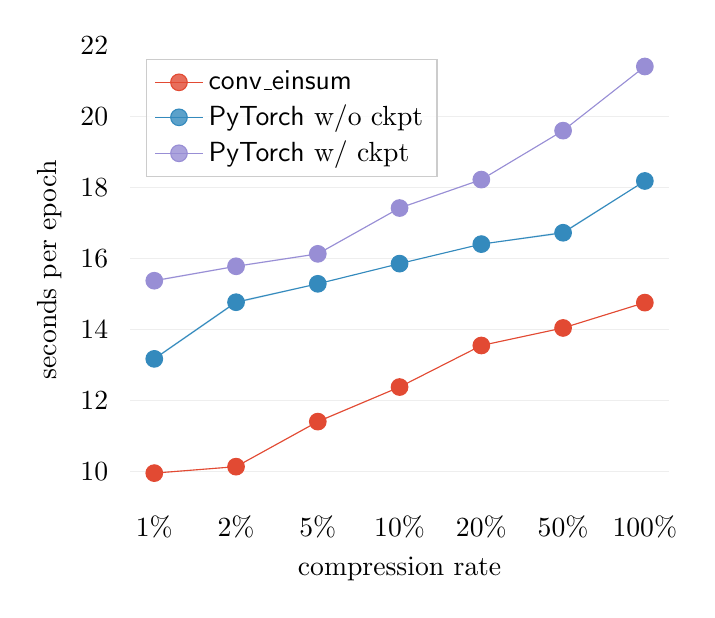
\begin{tikzpicture}

\definecolor{color0}{rgb}{0.886274509803922,0.290196078431373,0.2}
\definecolor{color1}{rgb}{0.203921568627451,0.541176470588235,0.741176470588235}
\definecolor{color2}{rgb}{0.596078431372549,0.556862745098039,0.835294117647059}

\begin{axis}[
axis line style={white},
legend cell align={left},
legend style={
  fill opacity=0.8,
  draw opacity=1,
  text opacity=1,
  at={(0.03,0.97)},
  anchor=north west,
  draw=white!80!black
},
tick align=outside,
x grid style={white},
xlabel={compression rate},
xmajorticks=true,
xtick style={draw=none},
xmin=0.7, xmax=7.3,
xtick style={color=white!33.3333333333333!black},
xtick={0,1,2,3,4,5,6,7,8},
xticklabels={,1\%,2\%,5\%,10\%,20\%,50\%,100\%,},
y grid style={white!93.3333333333333!black},
ylabel={seconds per epoch},
ymajorgrids,
ymajorticks=true,
ytick style={draw=none},
ymin=9.37454510860963, ymax=22.0011356340453,
ytick style={color=white!33.3333333333333!black}
]
\path [fill=color0, fill opacity=0.2, very thin]
(axis cs:1,9.97888939594091)
--(axis cs:1,9.94848104158397)
--(axis cs:2,10.1341301651132)
--(axis cs:3,11.3958190917175)
--(axis cs:4,12.3763176840136)
--(axis cs:5,13.5476123502911)
--(axis cs:6,14.0413649796803)
--(axis cs:7,14.7558393319893)
--(axis cs:7,14.7805985649874)
--(axis cs:7,14.7805985649874)
--(axis cs:6,14.0654411776747)
--(axis cs:5,13.5710407997148)
--(axis cs:4,12.4026890609351)
--(axis cs:3,11.4390945371537)
--(axis cs:2,10.1600878148762)
--(axis cs:1,9.97888939594091)
--cycle;

\path [fill=color1, fill opacity=0.2, very thin]
(axis cs:1,13.212937010019)
--(axis cs:1,13.1535384683386)
--(axis cs:2,14.7450545267958)
--(axis cs:3,15.2850116246708)
--(axis cs:4,15.8561679766487)
--(axis cs:5,16.4046870752762)
--(axis cs:6,16.7053913914602)
--(axis cs:7,18.177804697754)
--(axis cs:7,18.2063369673803)
--(axis cs:7,18.2063369673803)
--(axis cs:6,16.7716333181007)
--(axis cs:5,16.42428094383)
--(axis cs:4,15.8744521810938)
--(axis cs:3,15.3123507003659)
--(axis cs:2,14.8091467188384)
--(axis cs:1,13.212937010019)
--cycle;

\path [fill=color2, fill opacity=0.2, very thin]
(axis cs:1,15.4098741636846)
--(axis cs:1,15.359715998838)
--(axis cs:2,15.7725788621953)
--(axis cs:3,16.1201950872304)
--(axis cs:4,17.4164371262628)
--(axis cs:5,18.2167318277783)
--(axis cs:6,19.6044257349086)
--(axis cs:7,21.4078674336427)
--(axis cs:7,21.4271997010709)
--(axis cs:7,21.4271997010709)
--(axis cs:6,19.6170218663005)
--(axis cs:5,18.2454027336093)
--(axis cs:4,17.4457221512634)
--(axis cs:3,16.1605883847617)
--(axis cs:2,15.8085988675863)
--(axis cs:1,15.4098741636846)
--cycle;

\addplot [color0, mark=*, mark size=3, mark options={solid}]
table {%
1 9.96550999752094
2 10.1470873850588
3 11.4158439723712
4 12.3896402537851
5 13.5595994157227
6 14.0536398303251
7 14.76731840598
};
\addlegendentry{\conveinsum}
\addplot [color1, mark=*, mark size=3, mark options={solid}]
table {%
1 13.1830173239945
2 14.7788677082024
3 15.2971175402266
4 15.8651858810578
5 16.4150359613708
6 16.7352038438847
7 18.1933125245181
};
\addlegendentry{\pytorch w/o ckpt}
\addplot [color2, mark=*, mark size=3, mark options={solid}]
table {%
1 15.3839614827876
2 15.7905301555126
3 16.1408722531031
4 17.4311567858633
5 18.2321026344214
6 19.6106560296321
7 21.4176957433932
};
\addlegendentry{\pytorch w/ ckpt}
\end{axis}

\end{tikzpicture}

    }
\subcaption{RCP Train}\label{fig:imagecls-rcp-vs-pytorch-train}
\vspace{-1em}
\end{minipage}%
\hfill
\begin{minipage}[b]{.5\linewidth}
\centering
\resizebox{\textwidth}{!}{
    % This file was created by tikzplotlib v0.9.8.
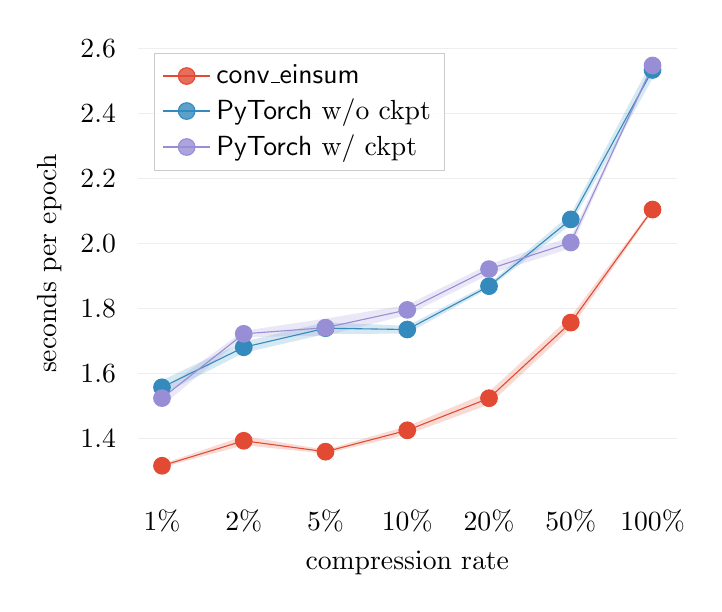
\begin{tikzpicture}

\definecolor{color0}{rgb}{0.886274509803922,0.290196078431373,0.2}
\definecolor{color1}{rgb}{0.203921568627451,0.541176470588235,0.741176470588235}
\definecolor{color2}{rgb}{0.596078431372549,0.556862745098039,0.835294117647059}

\begin{axis}[
axis line style={white},
legend cell align={left},
legend style={
  fill opacity=0.8,
  draw opacity=1,
  text opacity=1,
  at={(0.03,0.97)},
  anchor=north west,
  draw=white!80!black
},
tick align=outside,
x grid style={white},
xlabel={compression rate},
xmajorticks=true,
xtick style={draw=none},
xmin=0.7, xmax=7.3,
xtick style={color=white!33.3333333333333!black},
xtick={0,1,2,3,4,5,6,7,8},
xticklabels={,1\%,2\%,5\%,10\%,20\%,50\%,100\%,},
y grid style={white!93.3333333333333!black},
ylabel={seconds per epoch},
ymajorgrids,
ymajorticks=true,
ytick style={draw=none},
ymin=1.24857346169805, ymax=2.62702315020817,
ytick style={color=white!33.3333333333333!black},
ytick={1.2,1.4,1.6,1.8,2,2.2,2.4,2.6,2.8},
yticklabels={1.2,1.4,1.6,1.8,2.0,2.2,2.4,2.6,2.8}
]
\path [fill=color0, fill opacity=0.2, very thin]
(axis cs:1,1.32170128202879)
--(axis cs:1,1.31123026572124)
--(axis cs:2,1.37943586359388)
--(axis cs:3,1.35383196792479)
--(axis cs:4,1.4125147380759)
--(axis cs:5,1.5045691807526)
--(axis cs:6,1.73855847902859)
--(axis cs:7,2.09821307035801)
--(axis cs:7,2.11010459909695)
--(axis cs:7,2.11010459909695)
--(axis cs:6,1.77537474701384)
--(axis cs:5,1.54347203012721)
--(axis cs:4,1.43815583864567)
--(axis cs:3,1.3654502842472)
--(axis cs:2,1.40764016979432)
--(axis cs:1,1.32170128202879)
--cycle;

\path [fill=color1, fill opacity=0.2, very thin]
(axis cs:1,1.57928930643035)
--(axis cs:1,1.53615411385996)
--(axis cs:2,1.66334140504014)
--(axis cs:3,1.72147710695953)
--(axis cs:4,1.72265307494241)
--(axis cs:5,1.86189220791103)
--(axis cs:6,2.0579310830109)
--(axis cs:7,2.50675530494673)
--(axis cs:7,2.56436634618498)
--(axis cs:7,2.56436634618498)
--(axis cs:6,2.09045732611566)
--(axis cs:5,1.87629427307711)
--(axis cs:4,1.74657361604329)
--(axis cs:3,1.75756241081822)
--(axis cs:2,1.69808322827577)
--(axis cs:1,1.57928930643035)
--cycle;

\path [fill=color2, fill opacity=0.2, very thin]
(axis cs:1,1.547339830932)
--(axis cs:1,1.49956026530017)
--(axis cs:2,1.7118870869814)
--(axis cs:3,1.71640626028904)
--(axis cs:4,1.77963887616611)
--(axis cs:5,1.90444891921101)
--(axis cs:6,1.98507341910127)
--(axis cs:7,2.542796459306)
--(axis cs:7,2.55134724685929)
--(axis cs:7,2.55134724685929)
--(axis cs:6,2.02043206603775)
--(axis cs:5,1.93597701777938)
--(axis cs:4,1.81105152315929)
--(axis cs:3,1.76877109012378)
--(axis cs:2,1.73126280871942)
--(axis cs:1,1.547339830932)
--cycle;

\addplot [color0, mark=*, mark size=3, mark options={solid}]
table {%
1 1.31640031363155
2 1.39317822981615
3 1.35957493144292
4 1.42539200430426
5 1.52406284412461
6 1.75652346666184
7 2.10411776163085
};
\addlegendentry{\conveinsum}
\addplot [color1, mark=*, mark size=3, mark options={solid}]
table {%
1 1.55760821350578
2 1.68062363821
3 1.73921764819486
4 1.73527070724593
5 1.86857900731771
6 2.07382333450499
7 2.53333548435036
};
\addlegendentry{\pytorch w/o ckpt}
\addplot [color2, mark=*, mark size=3, mark options={solid}]
table {%
1 1.52429787768352
2 1.72205443814622
3 1.74087566195893
4 1.79565007027219
5 1.92109408585005
6 2.00270893324731
7 2.54707129726988
};
\addlegendentry{\pytorch w/ ckpt}
\end{axis}

\end{tikzpicture}

    }
\subcaption{RCP Test}\label{fig:imagecls-rcp-vs-pytorch-test}
\vspace{-1em}
\end{minipage}
\vspace{-1em}
\caption{\textbf{Runtime comparison between \conveinsum and \pytorch for an image classification task.} An RCP-TNN ($R=3$) is trained on the CIFAR-10 dataset. Runtimes are averaged over 3 random runs, and error bars are denoted by the shaded areas.}\label{fig:imagecls-rcp-vs-pytorch}
\vspace{-1em}
\end{figure}
\begin{figure}[!htbp]
\vspace{-1em}
\begin{minipage}[b]{.5\linewidth}
\centering
\resizebox{\textwidth}{!}{
   % This file was created by tikzplotlib v0.9.8.
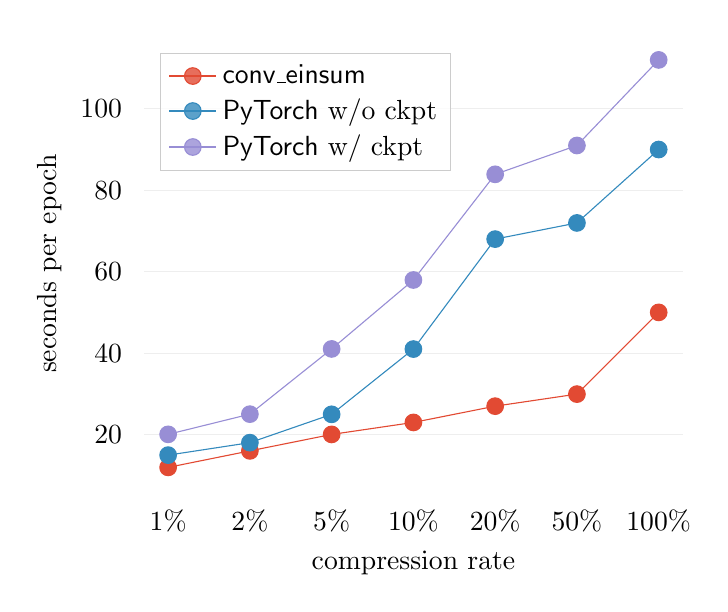
\begin{tikzpicture}

\definecolor{color0}{rgb}{0.886274509803922,0.290196078431373,0.2}
\definecolor{color1}{rgb}{0.203921568627451,0.541176470588235,0.741176470588235}
\definecolor{color2}{rgb}{0.596078431372549,0.556862745098039,0.835294117647059}

\begin{axis}[
axis line style={white},
legend cell align={left},
legend style={
  fill opacity=0.8,
  draw opacity=1,
  text opacity=1,
  at={(0.03,0.97)},
  anchor=north west,
  draw=white!80!black
},
tick align=outside,
x grid style={white},
xlabel={compression rate},
xmajorticks=true,
xtick style={draw=none},
xmin=0.7, xmax=7.3,
xtick style={color=white!33.3333333333333!black},
xtick={0,1,2,3,4,5,6,7,8},
xticklabels={,1\%,2\%,5\%,10\%,20\%,50\%,100\%,},
y grid style={white!93.3333333333333!black},
ylabel={seconds per epoch},
ymajorgrids,
ymajorticks=true,
ytick style={draw=none},
ymin=6.93387635391714, ymax=117.042037635885,
ytick style={color=white!33.3333333333333!black}
]
\path [fill=color0, fill opacity=0.2, very thin]
(axis cs:1,11.9579130614194)
--(axis cs:1,11.9387927758247)
--(axis cs:2,15.9987155814757)
--(axis cs:3,20.0414538754549)
--(axis cs:4,22.9731454322059)
--(axis cs:5,26.9623968234096)
--(axis cs:6,29.9266249782174)
--(axis cs:7,49.9866408536515)
--(axis cs:7,50.0456854259538)
--(axis cs:7,50.0456854259538)
--(axis cs:6,29.9706913551199)
--(axis cs:5,27.0099652497599)
--(axis cs:4,23.0030701756832)
--(axis cs:3,20.0482733902177)
--(axis cs:2,16.0087909500842)
--(axis cs:1,11.9579130614194)
--cycle;

\path [fill=color1, fill opacity=0.2, very thin]
(axis cs:1,14.9601884964392)
--(axis cs:1,14.9573120809723)
--(axis cs:2,18.0096463256373)
--(axis cs:3,24.9717105235957)
--(axis cs:4,40.9922461857787)
--(axis cs:5,67.9975861916329)
--(axis cs:6,71.9706864333012)
--(axis cs:7,90.0095730796352)
--(axis cs:7,90.0264998103663)
--(axis cs:7,90.0264998103663)
--(axis cs:6,71.9993267569562)
--(axis cs:5,68.0357558586188)
--(axis cs:4,41.0253107155279)
--(axis cs:3,24.9877007168248)
--(axis cs:2,18.0336335284603)
--(axis cs:1,14.9601884964392)
--cycle;

\path [fill=color2, fill opacity=0.2, very thin]
(axis cs:1,20.0659646338937)
--(axis cs:1,20.0561884908148)
--(axis cs:2,25.0081381260667)
--(axis cs:3,41.0301585519027)
--(axis cs:4,57.9443462099735)
--(axis cs:5,83.9158500404113)
--(axis cs:6,91.0043012476031)
--(axis cs:7,112.004011241764)
--(axis cs:7,112.037121213977)
--(axis cs:7,112.037121213977)
--(axis cs:6,91.0095831652896)
--(axis cs:5,83.9318453715774)
--(axis cs:4,58.0032027754974)
--(axis cs:3,41.0479536319266)
--(axis cs:2,25.0361794402418)
--(axis cs:1,20.0659646338937)
--cycle;

\addplot [color0, mark=*, mark size=3, mark options={solid}]
table {%
1 11.9480175327258
2 16.0038067857586
3 20.0446011253
4 22.9882729454736
5 26.9851024659074
6 29.9471383813403
7 50.0157408489748
};
\addlegendentry{\conveinsum}
\addplot [color1, mark=*, mark size=3, mark options={solid}]
table {%
1 14.9587413171968
2 18.0223304023785
3 24.979922393153
4 41.0090258257895
5 68.0150502045868
6 71.9856278608343
7 90.01875715427
};
\addlegendentry{\pytorch w/o ckpt}
\addplot [color2, mark=*, mark size=3, mark options={solid}]
table {%
1 20.0608634404145
2 25.0230362321103
3 41.0389765054386
4 57.9744796747981
5 83.9241095501663
6 91.0067440371285
7 112.021099689054
};
\addlegendentry{\pytorch w/ ckpt}
\end{axis}

\end{tikzpicture}

    }
\subcaption{CP Train}\label{fig:speech-rcp-vs-pytorch-train}
\end{minipage}%
\hfill
\begin{minipage}[b]{.5\linewidth}
\centering
\resizebox{\textwidth}{!}{
    % This file was created by tikzplotlib v0.9.8.
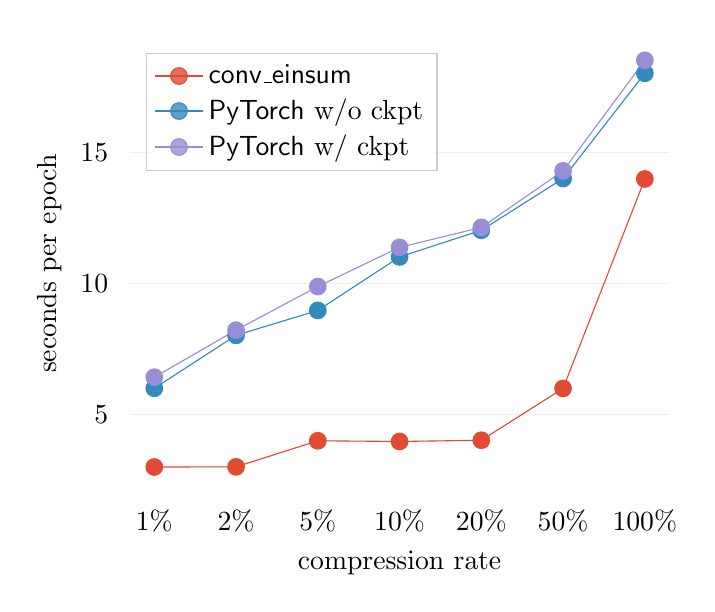
\begin{tikzpicture}

\definecolor{color0}{rgb}{0.886274509803922,0.290196078431373,0.2}
\definecolor{color1}{rgb}{0.203921568627451,0.541176470588235,0.741176470588235}
\definecolor{color2}{rgb}{0.596078431372549,0.556862745098039,0.835294117647059}

\begin{axis}[
axis line style={white},
legend cell align={left},
legend style={
  fill opacity=0.8,
  draw opacity=1,
  text opacity=1,
  at={(0.03,0.97)},
  anchor=north west,
  draw=white!80!black
},
tick align=outside,
x grid style={white},
xlabel={compression rate},
xmajorticks=true,
xtick style={draw=none},
xmin=0.7, xmax=7.3,
xtick style={color=white!33.3333333333333!black},
xtick={0,1,2,3,4,5,6,7,8},
xticklabels={,1\%,2\%,5\%,10\%,20\%,50\%,100\%,},
y grid style={white!93.3333333333333!black},
ylabel={seconds per epoch},
ymajorgrids,
ymajorticks=true,
ytick style={draw=none},
ymin=2.22512210560683, ymax=19.2968957549319,
ytick style={color=white!33.3333333333333!black}
]
\path [fill=color0, fill opacity=0.2, very thin]
(axis cs:1,3.02082834087343)
--(axis cs:1,3.01251180856302)
--(axis cs:2,3.00111181693979)
--(axis cs:3,4.00639642874174)
--(axis cs:4,3.97257409930328)
--(axis cs:5,4.02157149840141)
--(axis cs:6,5.9992105350004)
--(axis cs:7,13.9690904311333)
--(axis cs:7,14.0025188243429)
--(axis cs:7,14.0025188243429)
--(axis cs:6,6.02170121484232)
--(axis cs:5,4.04898502735233)
--(axis cs:4,4.00516644811893)
--(axis cs:3,4.02378492711419)
--(axis cs:2,3.04423841126161)
--(axis cs:1,3.02082834087343)
--cycle;

\path [fill=color1, fill opacity=0.2, very thin]
(axis cs:1,6.0366538238755)
--(axis cs:1,5.99205133823836)
--(axis cs:2,8.01488912462037)
--(axis cs:3,8.9645618694729)
--(axis cs:4,11.0102325304359)
--(axis cs:5,12.016898939181)
--(axis cs:6,13.9934676826971)
--(axis cs:7,17.9913456269073)
--(axis cs:7,18.0262259316063)
--(axis cs:7,18.0262259316063)
--(axis cs:6,14.0125760021348)
--(axis cs:5,12.0431994447087)
--(axis cs:4,11.023114466897)
--(axis cs:3,8.99385569759454)
--(axis cs:2,8.0437432830706)
--(axis cs:1,6.0366538238755)
--cycle;

\path [fill=color2, fill opacity=0.2, very thin]
(axis cs:1,6.46066041328354)
--(axis cs:1,6.40842164758021)
--(axis cs:2,8.2083759131759)
--(axis cs:3,9.86949595084347)
--(axis cs:4,11.3797587293601)
--(axis cs:5,12.1213207549009)
--(axis cs:6,14.2783842689879)
--(axis cs:7,18.4854525008877)
--(axis cs:7,18.5209060435989)
--(axis cs:7,18.5209060435989)
--(axis cs:6,14.309174118689)
--(axis cs:5,12.1619566188487)
--(axis cs:4,11.3825606425617)
--(axis cs:3,9.91010390628592)
--(axis cs:2,8.25026372301414)
--(axis cs:1,6.46066041328354)
--cycle;

\addplot [color0, mark=*, mark size=3, mark options={solid}]
table {%
1 3.01649832908809
2 3.0226706737841
3 4.01492994571654
4 3.98921456100731
5 4.03516300092398
6 6.01000819920187
7 13.985039344552
};
\addlegendentry{\conveinsum}
\addplot [color1, mark=*, mark size=3, mark options={solid}]
table {%
1 6.01426734372373
2 8.03024010547254
3 8.97909534125207
4 11.0167788677161
5 12.0316678376838
6 14.0029701561655
7 18.0082679228842
};
\addlegendentry{\pytorch w/o ckpt}
\addplot [color2, mark=*, mark size=3, mark options={solid}]
table {%
1 6.43605495595229
2 8.22935300451393
3 9.88988855120851
4 11.381229219844
5 12.1409493943312
6 14.2936303975075
7 18.5026482958735
};
\addlegendentry{\pytorch w/ ckpt}
\end{axis}

\end{tikzpicture}

    }
\subcaption{CP Test}\label{fig:speech-rcp-vs-pytorch-test}
\end{minipage}
\vspace{-2em}
\caption{\textbf{Run-time comparison between \conveinsum and \texttt{Pytorch} for a speech recognition task}. A CP-TNN is trained on the LibriSpeech dataset. Runtimes are averaged over 3 random runs, and error bars are denoted by the shaded areas.}\label{fig:speech-rcp-vs-pytorch}
\end{figure}
\begin{figure}[!htbp]
\vspace{-1em}
\begin{minipage}[b]{.5\linewidth}
\centering
\resizebox{\textwidth}{!}{
   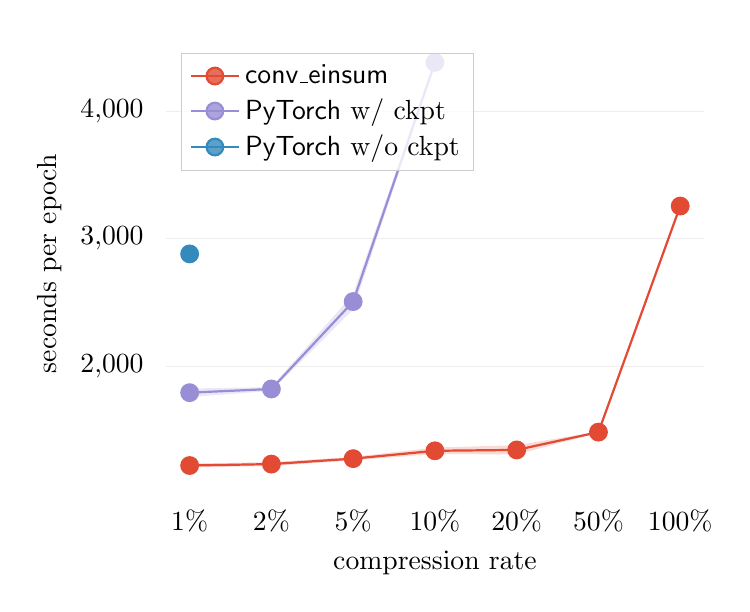
\begin{tikzpicture}

\definecolor{color0}{rgb}{0.886274509803922,0.290196078431373,0.2}
\definecolor{color2}{rgb}{0.203921568627451,0.541176470588235,0.741176470588235}
\definecolor{color1}{rgb}{0.596078431372549,0.556862745098039,0.835294117647059}

\begin{axis}[
axis line style={white},
legend cell align={left},
legend style={
  fill opacity=0.8,
  draw opacity=1,
  text opacity=1,
  at={(0.03, .97)},
  anchor=north west,
  draw=white!80!black
},
tick align=outside,
x grid style={white},
xlabel={compression rate},
xmajorticks=true,
xtick style={draw=none},
xmin=0.7, xmax=7.3,
xtick style={color=white!33.3333333333333!black},
xtick={0,1,2,3,4,5,6,7,8},
xticklabels={,1\%,2\%,5\%,10\%,20\%,50\%,100\%,},
y grid style={white!93.3333333333333!black},
ylabel={seconds per epoch},
ymajorgrids,
ymajorticks=true,
ytick style={draw=none},
ymin=1049.36179748519, ymax=4560.72815214266,
ytick style={color=white!33.3333333333333!black}
]
\path [fill=color0, fill opacity=0.2, very thin]
(axis cs:1,1239.52745899885)
--(axis cs:1,1208.96935906053)
--(axis cs:2,1219.52911242428)
--(axis cs:3,1264.72770568145)
--(axis cs:4,1314.11283386917)
--(axis cs:5,1310.60131838066)
--(axis cs:6,1481.39696673138)
--(axis cs:7,3240.75263688946)
--(axis cs:7,3272.38492714125)
--(axis cs:7,3272.38492714125)
--(axis cs:6,1489.5574229378)
--(axis cs:5,1382.84489640597)
--(axis cs:4,1364.69173989335)
--(axis cs:3,1291.67569619989)
--(axis cs:2,1250.89435414369)
--(axis cs:1,1239.52745899885)
--cycle;

\path [fill=color1, fill opacity=0.2, very thin]
(axis cs:1,1827.25514620111)
--(axis cs:1,1760.39553719911)
--(axis cs:2,1808.7589719549)
--(axis cs:3,2445.03883927714)
--(axis cs:4,4364.01023807436)
--(axis cs:4,4401.12059056732)
--(axis cs:4,4401.12059056732)
--(axis cs:3,2568.05167320782)
--(axis cs:2,1837.95356561557)
--(axis cs:1,1827.25514620111)
--cycle;

\path [fill=color2, fill opacity=0.2, very thin]
(axis cs:1,2913.93184443683)
--(axis cs:1,2848.5072446472)
--(axis cs:1,2913.93184443683)
--(axis cs:1,2913.93184443683)
--cycle;

\addplot [thick, color0, mark=*, mark size=3, mark options={solid}]
table {%
1 1223.9308060529
2 1235.17065172457
3 1277.74342014746
4 1339.26823402275
5 1346.10656586897
6 1485.5358628964
7 3256.12842998683
};
\addlegendentry{\conveinsum}
\addplot [thick, color1, mark=*, mark size=3, mark options={solid}]
table {%
1 1794.62780300269
2 1823.52637473414
3 2507.87693680823
4 4381.0754354547
};
\addlegendentry{\pytorch w/ ckpt}
\addplot [thick, color2, mark=*, mark size=3, mark options={solid}]
table {%
1 2881.26383770777
};
\addlegendentry{\pytorch  w/o ckpt}
\end{axis}

\end{tikzpicture}
    }
\subcaption{RCP Train (spatial)}\label{fig:video-rcp-vs-pytorch-train-spatial}
\end{minipage}%
\hfill
\begin{minipage}[b]{.5\linewidth}
\centering
\resizebox{\textwidth}{!}{
    % This file was created by tikzplotlib v0.9.8.
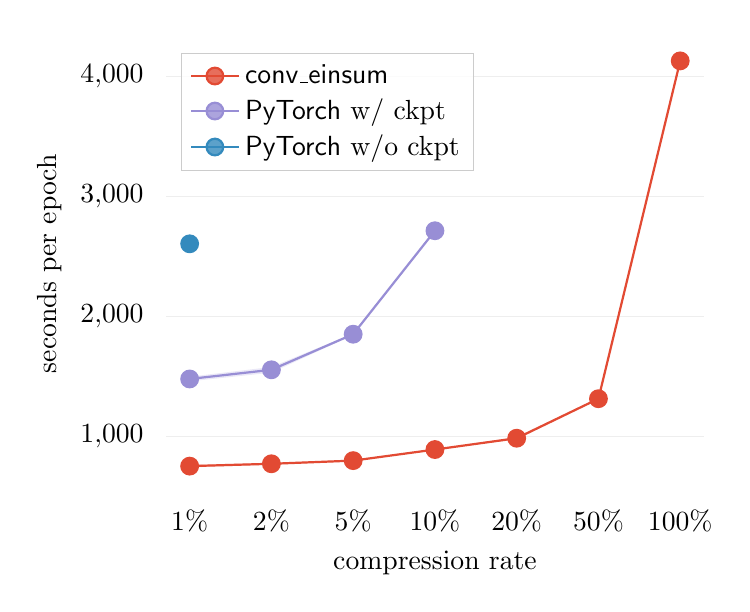
\begin{tikzpicture}

\definecolor{color0}{rgb}{0.886274509803922,0.290196078431373,0.2}
\definecolor{color2}{rgb}{0.203921568627451,0.541176470588235,0.741176470588235}
\definecolor{color1}{rgb}{0.596078431372549,0.556862745098039,0.835294117647059}

\begin{axis}[
axis line style={white},
legend cell align={left},
legend style={
  fill opacity=0.8,
  draw opacity=1,
  text opacity=1,
  at={(0.03, .97)},
  anchor=north west,
  draw=white!80!black
},
tick align=outside,
x grid style={white},
xlabel={compression rate},
xmajorticks=true,
xtick style={draw=none},
xmin=0.7, xmax=7.3,
xtick style={color=white!33.3333333333333!black},
xtick={0,1,2,3,4,5,6,7,8},
xticklabels={,1\%,2\%,5\%,10\%,20\%,50\%,100\%,},
y grid style={white!93.3333333333333!black},
ylabel={seconds per epoch},
ymajorgrids,
ymajorticks=true,
ytick style={draw=none},
ymin=569.971466073411, ymax=4308.63072954234,
ytick style={color=white!33.3333333333333!black}
]
\path [fill=color0, fill opacity=0.2, very thin]
(axis cs:1,762.306239838883)
--(axis cs:1,739.910523503816)
--(axis cs:2,763.074564933797)
--(axis cs:3,789.492653098703)
--(axis cs:4,887.874895808931)
--(axis cs:5,972.644076023388)
--(axis cs:6,1304.93861951356)
--(axis cs:7,4122.0327110838)
--(axis cs:7,4138.69167211193)
--(axis cs:7,4138.69167211193)
--(axis cs:6,1320.86505331794)
--(axis cs:5,995.159153544717)
--(axis cs:4,890.361982982634)
--(axis cs:3,803.373229607015)
--(axis cs:2,777.384986915317)
--(axis cs:1,762.306239838883)
--cycle;

\path [fill=color1, fill opacity=0.2, very thin]
(axis cs:1,1496.55048084937)
--(axis cs:1,1457.65330565694)
--(axis cs:2,1530.22273459423)
--(axis cs:3,1844.85296048969)
--(axis cs:4,2707.86924717783)
--(axis cs:4,2719.43859059785)
--(axis cs:4,2719.43859059785)
--(axis cs:3,1856.21068725365)
--(axis cs:2,1577.76604877951)
--(axis cs:1,1496.55048084937)
--cycle;

\path [fill=color2, fill opacity=0.2, very thin]
(axis cs:1,2612.0985164882)
--(axis cs:1,2597.19022640012)
--(axis cs:1,2612.0985164882)
--(axis cs:1,2612.0985164882)
--cycle;

\addplot [thick, color0, mark=*, mark size=3, mark options={solid}]
table {%
1 750.883967776807
2 770.309357175781
3 796.727914231485
4 889.107208063332
5 983.561759136815
6 1312.90264605939
7 4130.13177181716
};
\addlegendentry{\conveinsum}
\addplot [thick, color1, mark=*, mark size=3, mark options={solid}]
table {%
1 1477.65929167555
2 1554.07095801219
3 1850.86765552539
4 2713.68764614659
};
\addlegendentry{\pytorch w/ ckpt}
\addplot [thick, color2, mark=*, mark size=3, mark options={solid}]
table {%
1 2604.73291728878
};
\addlegendentry{\pytorch  w/o ckpt}
\end{axis}

\end{tikzpicture}
    }
\subcaption{RCP Test (spatial)}\label{fig:video-rcp-vs-pytorch-test-spatial}
\end{minipage}
\begin{minipage}[b]{.5\linewidth}
\centering
\resizebox{\textwidth}{!}{
   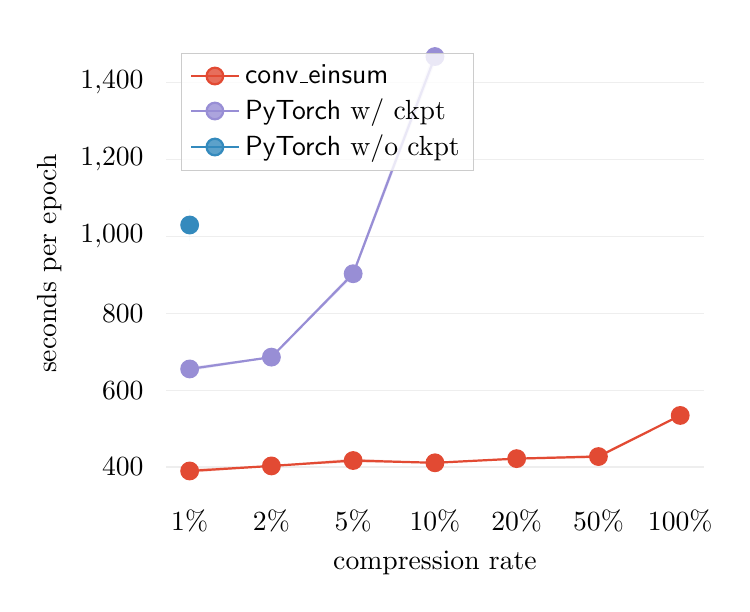
\begin{tikzpicture}

\definecolor{color0}{rgb}{0.886274509803922,0.290196078431373,0.2}
\definecolor{color2}{rgb}{0.203921568627451,0.541176470588235,0.741176470588235}
\definecolor{color1}{rgb}{0.596078431372549,0.556862745098039,0.835294117647059}

\begin{axis}[
axis line style={white},
legend cell align={left},
legend style={
  fill opacity=0.8,
  draw opacity=1,
  text opacity=1,
  at={(0.03, .97)},
  anchor=north west,
  draw=white!80!black
},
tick align=outside,
x grid style={white},
xlabel={compression rate},
xmajorticks=true,
xtick style={draw=none},
xmin=0.7, xmax=7.3,
xtick style={color=white!33.3333333333333!black},
xtick={0,1,2,3,4,5,6,7,8},
xticklabels={,1\%,2\%,5\%,10\%,20\%,50\%,100\%,},
y grid style={white!93.3333333333333!black},
ylabel={seconds per epoch},
ymajorgrids,
ymajorticks=true,
ytick style={draw=none},
ymin=346, ymax=1512,
ytick style={color=white!33.3333333333333!black}
]

\path [fill=color0, fill opacity=0.2, very thin]
(axis cs:1,394.994080571972)
--(axis cs:1,384.670112207607)
--(axis cs:2,401.557716590471)
--(axis cs:3,411.985227716121)
--(axis cs:4,410.301454913171)
--(axis cs:5,419.494550377922)
--(axis cs:6,423.325225105356)
--(axis cs:7,532.779729431467)
--(axis cs:7,535.549289999917)
--(axis cs:7,535.549289999917)
--(axis cs:6,431.521942897768)
--(axis cs:5,424.466288947851)
--(axis cs:4,411.648972176981)
--(axis cs:3,422.433903950399)
--(axis cs:2,404.25287990618)
--(axis cs:1,394.994080571972)
--cycle;

\path [fill=color1, fill opacity=0.2, very thin]
(axis cs:1,660.375275012558)
--(axis cs:1,649.571725671742)
--(axis cs:2,684.202231056962)
--(axis cs:3,895.361167953714)
--(axis cs:4,1450.24732870974)
--(axis cs:4,1487.16655882353)
--(axis cs:4,1487.16655882353)
--(axis cs:3,910.1473574649)
--(axis cs:2,687.550471411229)
--(axis cs:1,660.375275012558)
--cycle;

\path [fill=color2, fill opacity=0.2, very thin]
(axis cs:1,1071.73637097018)
--(axis cs:1,987.822122059148)
--(axis cs:1,1071.73637097018)
--(axis cs:1,1071.73637097018)
--cycle;

\addplot [thick, color0, mark=*, mark size=3, mark options={solid}]
table {%
1 389.78569338716
2 402.87011214031
3 416.952379424285
4 411.028575204281
5 421.904832880723
6 427.309693358374
7 534.177028678868
};
\addlegendentry{\conveinsum}
\addplot [thick, color1, mark=*, mark size=3, mark options={solid}]
table {%
1 655.121269077282
2 685.848327625873
3 902.77300224698
4 1467.62335191017
};
\addlegendentry{\pytorch w/ ckpt}
\addplot [thick, color2, mark=*, mark size=3, mark options={solid}]
table {%
1 1029.50275621723
};
\addlegendentry{\pytorch w/o ckpt}
\end{axis}

\end{tikzpicture}
    }
\subcaption{RCP Train (temporal)}\label{fig:video-rcp-vs-pytorch-train-temporal}
\vspace{-1em}
\end{minipage}%
\hfill
\begin{minipage}[b]{.5\linewidth}
\centering
\resizebox{\textwidth}{!}{
    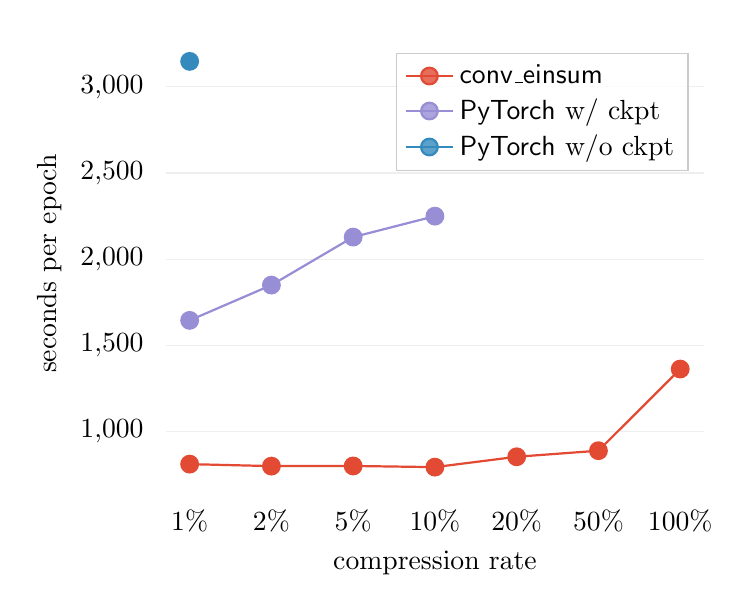
\begin{tikzpicture}

\definecolor{color0}{rgb}{0.886274509803922,0.290196078431373,0.2}
\definecolor{color2}{rgb}{0.203921568627451,0.541176470588235,0.741176470588235}
\definecolor{color1}{rgb}{0.596078431372549,0.556862745098039,0.835294117647059}

\begin{axis}[
axis line style={white},
legend cell align={left},
legend style={
  fill opacity=0.8,
  draw opacity=1,
  text opacity=1,
  at={(0.97, .97)},
  anchor=north east,
  draw=white!80!black
},
tick align=outside,
x grid style={white},
xlabel={compression rate},
xmajorticks=true,
xtick style={draw=none},
xmin=0.7, xmax=7.3,
xtick style={color=white!33.3333333333333!black},
xtick={0,1,2,3,4,5,6,7,8},
xticklabels={,1\%,2\%,5\%,10\%,20\%,50\%,100\%,},
y grid style={white!93.3333333333333!black},
ylabel={seconds per epoch},
ymajorgrids,
ymajorticks=true,
ytick style={draw=none},
ymin=672.920680442213, ymax=3274.58995911469,
ytick style={color=white!33.3333333333333!black}
]
\path [fill=color0, fill opacity=0.2, very thin]
(axis cs:1,811.197211734943)
--(axis cs:1,809.311383559561)
--(axis cs:2,797.680837493999)
--(axis cs:3,797.891855126853)
--(axis cs:4,791.178374927326)
--(axis cs:5,850.354460571758)
--(axis cs:6,887.096614639351)
--(axis cs:7,1361.09427982447)
--(axis cs:7,1363.19545041028)
--(axis cs:7,1363.19545041028)
--(axis cs:6,889.354224874219)
--(axis cs:5,855.87117788804)
--(axis cs:4,794.946955823782)
--(axis cs:3,801.557386907425)
--(axis cs:2,800.036214932191)
--(axis cs:1,811.197211734943)
--cycle;

\path [fill=color1, fill opacity=0.2, very thin]
(axis cs:1,1648.08090269321)
--(axis cs:1,1640.80047986953)
--(axis cs:2,1843.43954292875)
--(axis cs:3,2123.77688430585)
--(axis cs:4,2245.53010930735)
--(axis cs:4,2253.40970882798)
--(axis cs:4,2253.40970882798)
--(axis cs:3,2132.33727578151)
--(axis cs:2,1855.20582699139)
--(axis cs:1,1648.08090269321)
--cycle;

\path [fill=color2, fill opacity=0.2, very thin]
(axis cs:1,3156.33226462958)
--(axis cs:1,3137.35956281991)
--(axis cs:1,3156.33226462958)
--(axis cs:1,3156.33226462958)
--cycle;

\addplot [thick, color0, mark=*, mark size=3, mark options={solid}]
table {%
1 810.286726909255
2 798.830193285604
3 799.659436504972
4 792.972112924258
5 853.007709490447
6 888.249353679901
7 1362.07882422257
};
\addlegendentry{\conveinsum}
\addplot [thick, color1, mark=*, mark size=3, mark options={solid}]
table {%
1 1644.46058021686
2 1849.39908427744
3 2127.90901954
4 2249.39714615065
};
\addlegendentry{\pytorch w/ ckpt}
\addplot [thick, color2, mark=*, mark size=3, mark options={solid}]
table {%
1 3147.53106714877
};
\addlegendentry{\pytorch  w/o ckpt}
\end{axis}

\end{tikzpicture}
    }
\subcaption{RCP Test (temporal)}\label{fig:video-rcp-vs-pytorch-test-temporal}
\vspace{-1em}
\end{minipage}
\caption{\textbf{Run-time comparison between \conveinsum and \pytorch for a video classification machine learning task} An RCP-TNN ($R=3$) is trained on the UCF-101 dataset. All tests were run using the maximum allowable batch size. \pytorch w/ checkpointing was only able to run without memory overflow for compression rates 1\% - 10\% and \pytorch w/o checkpointing was only able to run without memory overflow for compression rate 1\%. Runtimes are averaged over 3 random runs, and error bars are denoted by the shaded areas. }\label{fig:video-rcp-vs-pytorch}
\vspace{-1em}
\end{figure}

\emph{(1) The optimal sequencer used in \conveinsum significantly improves the runtime efficiency of training and test in TNNs.} 
In \Cref{fig:imagecls-rcp-vs-pytorch,fig:speech-rcp-vs-pytorch,fig:video-rcp-vs-pytorch}, we compare the training and test times between \conveinsum and \pytorch (with and w/o checkpointing) implementations over a wide range of model scales and using different forms of tensor decomposition. The IC and VC tasks use RCP decompositions, while the ASR task uses a standard CP decomposition. 
We observe that \conveinsum universally outperforms the baselines. In the VC task, for each model size, we use the maximal allowable batch size, while in the ASR task, we compare implementations using the same batch size. Furthermore, in \Cref{tab:different-tensor-forms} we show that \conveinsum outperforms \pytorch in the IC task under different tensor decompositions.
We observe that when memory requirement is the bottleneck of a task (such as VC), checkpointing helps accelerate the runtime by alleviating potential memory overflows and allowing more batches. On the other hand, when the batch sizes are the same (as in ASR), checkpointing itself trades computational complexity for space, thus increasing the overall runtime. In either scenario, \conveinsum achieves the fastest runtimes in all tasks compared to \pytorch implementations with and without checkpointing.

\emph{(2) \autotnn works for weight tensors with different sizes.}
\autotnn serves as a general efficient library solution and is tensor-structure-agnostic. The networks we have experimented with contain weights of vastly differing sizes. As shown in \Cref{fig:imagecls-rcp-vs-pytorch,fig:speech-rcp-vs-pytorch,fig:video-rcp-vs-pytorch}, \autotnn exhibits competitive results against existing \pytorch solutions (with or without) checkpointing over various tensor sizes.

\emph{(3) \autotnn works for a variety of tensor forms.}
\conveinsum is both data-agnostic and structure-agnostic. Given any sequence of multilinear tensor operations, \conveinsum computes the optimal sequence with least number of FLOPs. As a result, \conveinsum is a universal solution to training any TNN. \Cref{tab:different-tensor-forms} in \Cref{app:experiments} shows the results of the image classification task on CIFAR10 using different forms of tensor decomposition. We could observe that \conveinsum outperforms \pytorch with/without checkpointing in all cases. 

\section{Conclusions and Discussions}
\label{sec:conclusion}

In this paper, we introduce an open-source library \autotnn, which is capable of building and efficiently training TNNs. Our \autotnn is competitive against and in many cases, superior to \pytorch TNN training.
For future work, we plan to further accelerate training and test times through incorporation of parallel computation paradigms into the intra-layer tensor computations. {Since our \autotnn relies on the \pytorch backend, we can also use tensorRT to further accelerate OpenTNN. Additionally, we will investigate incorporating quantization, pruning, and knowledge distillation techniques directly into \autotnn.}

\newpage
\bibliography{\bibhome/supp_bib}
\bibliographystyle{\inchome/icml2022}

\clearpage
\appendix

% \begin{center}
% {\bf \Large Appendices for \papertitle}
% \end{center}

\section{Additional Related Work}\label{app:add_related_work}


\textbf{Tensor networks.}
Tensor networks are widely used in quantum physics~\citep{orus2014practical}, 
numerical analysis~\citep{grasedyck2013literature}, and machine learning~\citep{cichocki2016tensor,cichocki2017tensor}. 
In neural networks, \citet{cohen2016convolutional} and \citet{khrulkov2018expressive} 
use tensor networks to prove the expressive power of convolutional and recurrent neural networks. Recently, \citet{hayashi2019exploring} combine tensor networks with genetic algorithms to search for efficient layer designs.
However, traditional tensor networks do not support {\em convolutions} in their operations, which is essential in convolutional neural networks. 
\section{Supplementary Material for Tensor Operations and \einsum}
\label{app:A1multi}

\subsection{Examples of primitive operations}\label{app:subsec:einsum}

% 1) Tensor contraction
\textbf{Contraction.}
{\em Tensor contraction} generalizes matrix multiplication to higher-order tensors. 
For instance, given two $3^\rd$ order tensors $\tensorSup{T}{1} \in \R^{A \times B \times C}, \tensorSup{T}{2} \in \R^{A \times D \times E}$, we can define a contraction between the modes with shared dimension size $A$. The operation returns a $4^\th$ order tensor $\tensor{T} \in \R^{B \times C \times D \times E}$ with its entries calculated as:
%\begin{equation}
%\label{eq:contraction}
$\tensorSub{T}{b,c,d,e} = \sum_{a = 1}^{A}
\tensorInd{T}{1}{a,b,c} \cdot \tensorInd{T}{2}{a,d,e}$.
%\end{equation}
This contraction would be submitted to \einsum as:
\begin{lstlisting}
T = einsum("abc,ade->bcde", T1, T2)
\end{lstlisting}
\vspace{-1em}
Here, the modes are ordered and represented by concatenated letters (which can be case-sensitive). These sub-strings, corresponding to each input tensor, are separated by commas and lie to the left of the arrow. The output, which lies to the right of the arrow, concatenates all mode letters in a single string sans the letter $\textsf{"a"}$ to indicate that a contraction must occur over these modes. The remaining parameters correspond to the ordered set of tensors. This method will fail if the modes denoted by the same letters do not share dimension sizes. So a contraction corresponds to a letter that appears in all inputs, but not the output.

% 2) Tensor outer product
\textbf{Outer product.}
{\em Tensor outer product} generalizes outer product to higher-order tensors. For instance, an outer product of two $3^\rd$ order tensors $\tensorSup{T}{1} \in \R^{A \times B \times C}, \tensorSup{T}{2} \in \R^{D \times E \times F}$ returns a $6^\th$ order tensor $\tensor{T} \in \R^{A \times B \times C \times D \times E \times F}$. The entries of $\tensor{T}$ are calculated as:
%\begin{equation}
%\label{eq:outer-product}
$\tensorSub{T}{a,b,c,d,e,f} =
\tensorInd{T}{1}{a,b,c} \cdot
\tensorInd{T}{2}{d,e,f}$.
%\end{equation}
In the language of \einsum, we write this as:
\begin{lstlisting}
T = einsum("abc,def->abcdef", T1, T2)
\end{lstlisting}
\vspace{-1em}
Notice that a letter for the outer product only appears in one of the inputs and in the output.

% 3) Tensor batch product
\textbf{Batch product.}
{\em Tensor batch product} is a variation of the outer product. Given tensors $\tensorSup{T}{1} \in \R^{A \times B \times C}, \tensorSup{T}{2} \in \R^{C \times E \times D}$, the batch product over the dimensional-shared mode $C$ returns a $5^\th$ order tensor $\tensor{T}\in\R^{A \times B \times C \times D \times E}$. The entries of $\tensor{T}$ are calculated as:
%\begin{equation}
%\label{eq:batch-product}
$\tensorSub{T}{a,b,c,d,e} =
\tensorInd{T}{1}{a,b,c} \cdot
\tensorInd{T}{2}{a,d,e}$.
%\end{equation}
The \einsum implementation is
\begin{lstlisting}
T = einsum("abc,cde->abcde", T1, T2)
\end{lstlisting}
\vspace{-1em}
Notice that the letter corresponding to the batch product appears in both inputs and the output.



In this section, we will outline the multi-linear operations covered in \Cref{sec:preliminary} in full generality along with their \conveinsum representations and other tensor decompositions of TNNs. Much of this content adapts and follows the notation of \citet{su2018tensorial}.

\subsection{Fully General Multilinear operations} 
\label{app-sub:multiops}


% Multi-operations among multiple tensors
\textbf{Multi-operations among multiple tensors.}
We can simultaneously perform a series of multi-linear operations among a group of tensors.
Let $\tensorSup{T}{1} \in \R^{I \times T \times S}$,
$\tensorSup{T}{2} \in \R^{J \times R \times T}$, and
$\tensorSup{T}{3} \in \R^{K \times S \times R}$. We can define a simultaneous contraction on modes with dimension sizes $R, S,$ and $T$.
This simultaneous contraction returns a $3^\rd$ order tensor $\tensor{T} \in \R^{I \times J \times K}$, with its entries computed as
\begin{equation}
\label{eq:multi-operation-2}
\tensorSub{T}{i,j,k} = \sum_{r = 1}^{R} \sum_{s = 1}^{S} \sum_{t = 1}^{T} 
\tensorInd{T}{1}{i,t,s} \tensorInd{T}{2}{j,r,t} \tensorInd{T}{3}{k,s,r}
\end{equation}
Equivalently, via \conveinsum, we can write it as:
\begin{lstlisting}
T = conv_einsum("its,jrt,ksr->ijk", T1, T2, T3)
\end{lstlisting}
\vspace{-1em}
% In Appendix~\ref{multiops}, 
Below we outline a simpler example that performs multiple operations between two tensors.


% Table for primitive operations
\begin{table*}[!htbp]
\centering
\resizebox{\textwidth}{!}{
\setlength{\tabcolsep}{3pt}
\begin{tabular}{c| c |c}
\toprule
Operation & Definition & \conveinsum \\
\midrule
	% 1) tensor contraction
	\begin{tabular}{l} mode-($k, l$) \\ Tensor Contraction \end{tabular} & 
	\begin{tabular}{l} $\tensor{T}_{i_0, \cdots, i_{k-1}, i_{k+1}, \cdots, i_{m-1}, j_0, \cdots, j_{l-1}, j_{l+1}, \cdots, j_{n-1}}$ \\
	$ = \big< \tensorSup{T}{0}_{i_0, \cdots, i_{k-1},{ :}, i_{k+1}, \cdots, i_{m-1}},  \tensorSup{T}{1}_{j_0, \cdots, j_{l-1}, {:}, j_{l+1}, \cdots, j_{n-1}}\big>$ \\ 
	\end{tabular} & \begin{tabular}{l} $\textcolor{red}{I_0 \cdots I_{k-1} I_k \cdots I_{m-1}}, \textcolor{blue}{J_0 \cdots J_{l-1} J_l \cdots J_{n-1}}$ \\ $\rightarrow  I_{1} I_{k-1} I_{k+1} I_{m-1} J_0 \cdots J_{l-1} J_{l+1} \cdots J_{n-1}$ \end{tabular}\\
\midrule
	% 2) tensor convolution
	\begin{tabular}{l} mode-$(k, l)$ \\Tensor Convolution \end{tabular} & 
	\begin{tabular}{l}$\tensorInd{T}{i_0, \cdots, i_{k-1}, {:}, i_{k+1}, \cdots, i_{m-1}, j_0, \cdots, j_{l-1}, j_{l+1}, \cdots, j_{n-1}}{2} $ \\
	$= \tensorSup{T}{0}_{i_0, \cdots, i_{k-1}, {:}, i_{k+1}, \cdots, i_{m-1}} \ast \tensorSup{T}{1}_{j_0, \cdots, j_{l-1},{ :}, j_{l+1}, \cdots, j_{n-1}}$ \\ 
	 \end{tabular} & \begin{tabular}{l} $\textcolor{red}{I_0 \cdots I_{k-1} C \cdots I_{m-1}}, \textcolor{blue}{J_0 \cdots J_{l-1} C \cdots J_{n-1}}$ \\ $\rightarrow  I_{1} I_{k-1} C I_{k+1} I_{m-1} J_0 \cdots J_{l-1} J_{l+1} \cdots J_{n-1} \mid C$ \end{tabular}\\
\midrule
	% 3) tensor batch product
	\begin{tabular}{l} mode-($k, l$) \\ Tensor Batch Product \end{tabular} &
	\begin{tabular}{l} $\tensor{T}_{i_0, \cdots, i_{k-1}, {r}, i_{k+1}, \cdots, i_{m-1}, j_0, \cdots,  j_{n-1}} $ \\
	$=\tensorSup{T}{0}_{i_0, \cdots, i_{k-1}, {r}, i_{k+1}, \cdots, i_{m-1}} ~ \tensorSup{T}{1}_{j_0, \cdots, j_{l-1},{ r}, j_{l+1}, \cdots, j_{n-1}}$ \\ 
	\end{tabular} & \begin{tabular}{l} $\textcolor{red}{I_0 \cdots I_{k-1} C \cdots I_{m-1}}, \textcolor{blue}{J_0 \cdots J_{l-1} J_l \cdots J_{n-1}}$ \\ $\rightarrow  I_{1} I_{k-1} I_k I_{k+1} I_{m-1} J_0 \cdots J_{l-1} J_{l+1} \cdots J_{n-1}$  \end{tabular}\\
\midrule
	% 2) tensor outer product
	\begin{tabular}{l} Tensor Outer Product \end{tabular} & 
	\begin{tabular}{l}  $\tensorSup{T}{0}_{i_0, \cdots, i_{k-1}, i_k, i_{k+1}, \cdots, i_{m-1}, j_0, \cdots, j_{l-1}, j_l, j_{l+1}, \cdots, j_{n-1}}$ \\
	$= \tensorSup{T}{1}_{i_0, \cdots, i_{m-1}} \ast \tensorSub{Y}{j_0, \cdots, j_{l+1}, \cdots, j_{n-1}}$ \\ 
	 \end{tabular} &
	 \begin{tabular}{l} $\textcolor{red}{I_0 \cdots I_{m-1}}, \textcolor{blue}{J_0 \cdots J_{n-1}}$ \\ $\rightarrow  I_{1} \cdots I_{m-1} J_0 \cdots J_{n-1}$  \end{tabular}\\
\bottomrule
\end{tabular}
}
\caption{\textbf{Primitive tensor operations}. 
$\tensorSup{T}{0} \in \R^{I_0 \times \cdots \times I_{m-1}}, 
\tensorSup{T}{1} \in \R^{J_0 \times \cdots \times J_{n-1}}$ are the input tensors and
$\tensor{T}$ is the output tensor.
Note that both mode-$(I_k, J_l)$ tensor contraction, mode-($I_k, J_l$) tensor batch product 
are legal only if $I_k = J_l$. The outer product can be performed with any two tensors. Red highlighted modes are owned by $\tensorSup{T}{0}$ while blue highlighted modes belong to $\tensorSup{T}{1}$.}
\label{tab:primitive-operations}
\end{table*}

% (1) Tensor contraction
\paragraph{Tensor contraction} 
Given tensors $\tensorSup{T}{0}\in\mathbb{R}^{I_0 \times \cdots I_k \times I_{m-1}}, \tensorSup{T}{1}\in\mathbb{R}^{J_0 \times \cdots J_l  \cdots \times J_{n-1}}$, the mode-($k,l$) contraction returns an order $(m+n-2)$ tensor \\$\tensor{T}\in\mathbb{R}^{I_0\times\cdots I_{k-1} \times I_{k+1}\times \cdots \times I_{m-1}\times J_0 \times \cdots \times J_{l-1}\times J_{l+1}\times\cdots\times J_{n-1} }$. The entries of $\tensor{T}$ are calculated as follows: 
\begin{align*}
&\tensor{T}_{i_0, \cdots, i_{k-1}, i_{k+1}, \cdots, i_{m-1}, j_0, \cdots, j_{l-1}, j_{l+1}, \cdots, j_{n-1}}\\ &=\sum_{r=1}^{I_k-1}\tensorSup{T}{0}_{i_0, \cdots, i_{k-1},r, i_{k+1}, \cdots, i_{m-1}}\cdot  \tensorSup{T}{1}_{j_0, \cdots, j_{l-1}, r, j_{l+1}, \cdots, j_{n-1}}\\
&=\langle \tensorSup{T}{0}_{i_0, \cdots, i_{k-1},{ :}, i_{k+1}, \cdots, i_{m-1}},  \tensorSup{T}{1}_{j_0, \cdots, j_{l-1}, {:}, j_{l+1}, \cdots, j_{n-1}}\rangle.
\end{align*}

% (2) Tensor convolution
\paragraph{Tensor Convolution} 
Given tensors $\tensorSup{T}{0}\in\mathbb{R}^{I_0\times \cdots \times I_{m-1}}, \tensorSup{T}{1}\in\mathbb{R}^{J_0 \times \cdots \times J_{n-1}}$, the mode-($k,l$) convolution returns an order $(m+n-1)$ tensor \\$\tensor{T}\in\mathbb{R}^{I_0\times\cdots I'_k \times \cdots \times I_{m-1}\times J_0 \times \cdots \times J_{l-1}\times J_{l+1}\times\cdots\times J_{n-1}}$. For any convolution operator * the entries of $\tensor{T}$ are calculated as follows:
\begin{align*}
& \tensor{T}_{i_0, \cdots, i_{k-1}, {:}, i_{k+1}, \cdots, i_{m-1}, j_0, \cdots, j_{l-1}, j_{l+1}, \cdots, j_{n-1}} \\
	&= \tensorSup{T}{0}_{i_0, \cdots, i_{k-1}, {:}, i_{k+1}, \cdots, i_{m-1}} \ast \tensorSup{T}{1}_{j_0, \cdots, j_{l-1},{ :}, j_{l+1}, \cdots, j_{n-1}}\\
	&= \tensorSup{T}{1}_{j_0, \cdots, j_{l-1},{ :}, j_{l+1}, \cdots, j_{n-1}} \bar{\ast} \tensorSup{T}{0}_{i_0, \cdots, i_{k-1}, {:}, i_{k+1}, \cdots, i_{m-1}}
\end{align*}
Here we have intentionally left $\ast$ and the dimension of the $k$-th mode $I'_k$ ambiguous, as it will vary depending on the type of convolution specified by the user. For example, with max padding, we have that $I'_k=\max\{I_k,J_l\}$, and with same-padding we have $I'_k=I_k$. 

% (3) tensor batch product
\paragraph{Tensor Batch Product}
Given tensors $\tensorSup{T}{0}\in\mathbb{R}^{I_0\times \cdots I_{k} \cdots \times I_{m-1}}, \tensorSup{T}{1}\in\mathbb{R}^{J_0 \times \cdots I_l \cdots \times J_{n-1}}$, the mode-($k,l$) batch product returns an order $(m+n-1)$ tensor $\tensor{T}\in\mathbb{R}^{I_0\times\cdots I_k \times \cdots \times I_{m-1}\times J_0 \times \cdots \times \cdots\times J_{n-1}}$. The entries of $\tensor{T}$ are calculated as follows:
\begin{align*}
& \tensor{T}_{i_0, \cdots, i_{k-1}, r, i_{k+1}, \cdots, i_{m-1}, j_0, \cdots, j_{l-1}, j_{l+1}, \cdots, j_{n-1}} \\
	&= \tensorSup{T}{0}_{i_0, \cdots, i_{k-1}, r, i_{k+1}, \cdots, i_{m-1}} \tensorSup{T}{1}_{j_0, \cdots, j_{l-1},r, j_{l+1}, \cdots, j_{n-1}}
\end{align*}

% (4) tensor outer product
\paragraph{Tensor Outer Product}
 Given tensors $\tensorSup{T}{0}\in\mathbb{R}^{I_0\times \cdots \times I_{m-1}}, \tensorSup{T}{1}\in\mathbb{R}^{J_0 \times \cdots \times J_{n-1}}$, the outer product returns an order $(m+n)$ tensor $\tensor{T}\in\mathbb{R}^{I_0\times\cdots I_k \times \cdots \times I_{m-1}\times J_0 \times \cdots \times J_{n-1}}$. The entries of $\tensor{T}$ are calculated as follows:
\begin{align}
\tensor{T}_{i_0, \cdots, i_{m-1}, j_0, \cdots, j_{n-1}}
	&= \tensorSup{T}{0}_{i_0, \cdots, i_{m-1}} \tensorSup{T}{1}_{j_0, \cdots, j_{n-1}}.
\end{align}

\Cref{tab:primitive-operations} summarizes these multi-linear operations along with their \conveinsum input representations. 

\subsection{Tensorial Neural Networks}
\label{app-sub:TNN}

% 1) CP decomposition
\textbf{CP decomposition}~\citep{kolda2009tensor}.
(1a) In a {\em CP convolutional layer}~\citep{lebedev2015speeding}, the original kernel $\tensor{W} \in \R^{T \times S \times H \times W}$ is CP factorized as:
\begin{lstlisting}
W = conv_einsum("rt,rs,rh,rw->tshw", W1, W2, W3, W4).
\end{lstlisting}
\vspace{-0.5em}
As a result, the layer is parameterized by $4$ weight matrices $\matrixSup{W}{1} \in \R^{R \times T}$, $\matrixSup{W}{2} \in \R^{R \times S}$, $\matrixSup{W}{3} \in \R^{R \times H}$, $\matrixSup{W}{4} \in \R^{R \times W}$. We can write this layer in \conveinsum as
\begin{lstlisting}
Y = conv_einsum("bshw,rt,ts,rh,rw->bthw|hw", X, W1)
\end{lstlisting}
\vspace{-0.5em}

(1b) In a {\em reshaped CP convolutional layer}~\citep{su2018tensorial}, the original kernel $\mytensor{W}$ is first reshaped as $\mytensor{\overline{W}} \in \R^{T_1 \cdots \times T_M \times S_1 \cdots \times S_M \times H \times W}$ such that $T = \prod_{m = 1}^{M} T_m$ and $S = \prod_{m = 1}^{M} S_m$. Suppose $M = 3$, then the reshaped kernel is factorized by a CP decomposition as
\begin{lstlisting}
W = conv_einsum("r(t1)(s1),r(t2)(s2),r(t3)(s3),rhw->(t1)(t2)(t3)(s1)(s2)(s3)hw", W1, W2, W3, W0).
\end{lstlisting}
\vspace{-0.5em}
As a result, the layer is parameterized by $(M + 1)$ weight tensors $\tensorSup{W}{m} \in \R^{R \times T_m \times S_m}$ and $\tensorSup{W}{0} \in \R^{R \times H \times W}$. We can write the layer in \conveinsum as
\begin{lstlisting}
Y = conv_einsum("b(s1)(s2)(s3)hw,r(t1)(s1),r(t2)(s2),r(t3)(s3),rhw->b(t1)(t2)(t3)hw|hw", X, W1, W2, W3, W0)
\end{lstlisting}

% 2) Tucker decomposition 
\textbf{Tucker (TK) decomposition}~\citep{kolda2009tensor}.
(2a) In a {\em TK convolutional layer}~\citep{lebedev2015speeding}, the original kernel $\tensor{W} \in \R^{T \times S \times H \times W}$ is factorized by TK as:
\begin{lstlisting}
W = conv_einsum("(r1)t,(r2)s,(r1)(r2)hw->tshw", W1, W2, W0)
\end{lstlisting}
\vspace{-0.5em}
Consequently, the layer has $3$ weight tensors $\matrixSup{W}{1} \in \R^{R_1 \times T}$, $\matrixSup{W}{2} \in \R^{R_2 \times S}$, $\tensorSup{W}{0} \in \R^{R_1 \times R_2 \times H \times W}$ as parameters. We can write the layer in \conveinsum as
\begin{lstlisting}
Y = conv_einsum("bshw,(r1)t,(r2)s,(r1)(r2)hw->bthw|hw", X, W1, W2, W0)
\end{lstlisting}
\vspace{-0.5em}

(2b) In a {\em reshaped TK convolutional layer}~\citep{su2018tensorial}, the original kernel $\mytensor{W}$ is first reshaped as $\mytensor{\overline{W}} \in \R^{T_1 \cdots \times T_M \times S_1 \cdots \times S_M \times H \times W}$ such that $T = \prod_{m = 1}^{M} T_m$ and $S = \prod_{m = 1}^{M} S_m$. Suppose $M = 3$, the reshaped kernel is then factorized by a TK decomposition as
\begin{lstlisting}
W = conv_einsum("(r1)(t1)(s1),(r2)(t2)(s2),(r3)(t3)(s3),(r0)hw,(r0)(r1)(r2)(r3)->(t1)(t2)(t3)(s1)(s2)(s3)hw", W1, W2, W3, W0, C)
\end{lstlisting}
\vspace{-0.5em}
Therefore, the layer has $(M + 2)$ weight tensors $\tensorSup{W}{m} \in \R^{R \times T_m \times S_m}$, $\tensorSup{W}{0} \in \R^{R \times H \times W}$, $\tensor{C} \in \R^{R_0 \times R_1 \times R_2 \times R_3}$. We can write the layer in \conveinsum as
\begin{lstlisting}
Y = conv_einsum("b(s1)(s2)(s3)hw,(r1)(t1)(s1),(r2)(t2)(s2),(r3)(t3)(s3),(r0)hw,(r0)(r1)(r2)(r3)->b(t1)(t2)(t3)hw|hw", X, W1, W2, W3, W0, C)
\end{lstlisting}

% Tensor-Train decomposition
\textbf{Tensor-Train (TT) decomposition}~\citep{oseledets2011tensor}.
(3a) In a {\em TT convolutional layer}, the original kernel $\tensor{W} \in \R^{T \times S \times H \times W}$ is factorized by TT as:
\begin{lstlisting}
W = conv_einsum("(r1)t,(r1)(r2)h,(r2)(r3)w,(r3)s->tshw", W1, W2, W3, W4)
\end{lstlisting}
\vspace{-1em}
Consequently, the layer has $4$ weight tensors $\matrixSup{W}{1} \in \R^{R_1 \times T}$, $\matrixSup{W}{2} \in \R^{R_1 \times R_2 \times H}$, $\tensorSup{W}{3} \in \R^{R_2 \times R_3 \times W}$, and $\tensorSup{W}{4} \in \R^{R_3 \times S}$ as parameters. We can write the layer in \conveinsum as
\begin{lstlisting}
Y = conv_einsum("bshw,(r1)t,(r1)(r2)h,(r2)(r3)w,(r3)s->bthw|hw", X, W1, W2, W3, W4).
\end{lstlisting}
\vspace{-0.5em}

(3b) In a {\em reshaped TT convolutional layer}~\citep{garipov2016ultimate}, the original kernel $\mytensor{W}$ is first reshaped as $\mytensor{\overline{W}} \in \R^{T_1 \cdots \times T_M \times S_1 \cdots \times S_M \times H \times W}$ such that $T = \prod_{m = 1}^{M} T_m$ and $S = \prod_{m = 1}^{M} S_m$. Suppose $M = 3$, the reshaped kernel is then factorized by a TT decomposition as
\begin{lstlisting}
W = conv_einsum("(r1)(t1)(s1),(r1)(r2)(t2)(s2),(r2)(r3)(t3)(s3),(r3)hw->(t1)(t2)(t3)(s1)(s2)(s3)hw", W1, W2, W3, W0).
\end{lstlisting}
\vspace{-0.5em}
Therefore, the layer has $(M + 1)$ weight tensors $\tensorSup{W}{1} \in \R^{R_1 \times T_1 \times S_1}$, $\tensorSup{W}{m} \in \R^{R_{m - 1} \times R_m \times T_m \times S_m}$, and $\tensorSup{W}{0} \in \R^{R_3 \times H \times W}$. The layer in \conveinsum is
\begin{lstlisting}
Y = conv_einsum("b(s1)(s2)(s3)hw,(r1)(t1)(s1),(r1)(r2)(t2)(s2),(r2)(r3)(t3)(s3),(r3)hw->b(t1)(t2)(t3)hw|hw", X, W1, W2, W3, W0).
\end{lstlisting}

% Tensor-Ring decomposition
\textbf{Tensor-Ring (TR) decomposition}~\citep{zhao2016tensor}.
(4a) In a {\em TR convolutional layer}, the original kernel $\tensor{W} \in \R^{T \times S \times H \times W}$ is factorized by TR as:
\begin{lstlisting}
W = conv_einsum("(r0)(r1)t,(r1)(r2)h,(r2)(r3)w,(r3)(r0)s->tshw", W1, W2, W3, W4)
\end{lstlisting}
\vspace{-1em}
Consequently, the layer has $4$ weight tensors $\matrixSup{W}{1} \in \R^{R_1 \times T}$, $\matrixSup{W}{2} \in \R^{R_0 \times R_1 \times R_2 \times H}$, $\tensorSup{W}{3} \in \R^{R_2 \times R_3 \times W}$, and $\tensorSup{W}{4} \in \R^{R_3 \times R_0 \times S}$ as parameters. We can write the layer in \conveinsum as
\begin{lstlisting}
Y = conv_einsum("bshw,(r0)(r1)t,(r1)(r2)h,(r2)(r3)w,(r3)(r0)s->bthw|hw", X, W1, W2, W3, W4)
\end{lstlisting}
\vspace{-0.5em}

(4b) In a {\em reshaped TR convolutional layer}~\citep{su2018tensorial}, the original kernel $\mytensor{W}$ is first reshaped as $\mytensor{\overline{W}} \in \R^{T_1 \cdots \times T_M \times S_1 \cdots \times S_M \times H \times W}$ such that $T = \prod_{m = 1}^{M} T_m$ and $S = \prod_{m = 1}^{M} S_m$. Suppose $M = 3$, the reshaped kernel is then factorized by a TR decomposition as
\begin{lstlisting}
W = conv_einsum("(r0)(r1)(t1)(s1),(r1)(r2)(t2)(s2),(r2)(r3)(t3)(s3),(r3)(r0)hw->(t1)(t2)(t3)(s1)(s2)(s3)hw", W1, W2, W3, W0)
\end{lstlisting}
\vspace{-0.5em}
Therefore, the layer has $(M + 1)$ weight tensors $\tensorSup{W}{m} \in \R^{R_{m - 1} \times R_m \times T_m \times S_m}$, and $\tensorSup{W}{0} \in \R^{R_3 \times R_0 \times H \times W}$. The layer in \conveinsum is
\begin{lstlisting}
Y = conv_einsum("b(s1)(s2)(s3)hw,(r0)(r1)(t1)(s1),(r1)(r2)(t2)(s2),(r2)(r3)(t3)(s3),(r3)(r0)hw->b(t1)(t2)(t3)hw|hw", X, W1, W2, W3, W0)
\end{lstlisting}

\subsubsection{Efficient Convolutional Layers} \label{app:efficientNN}
A number of works design efficient convolutional layers by modifying the linear operations in deep networks. These types of convolutional layers can be thought as special cases of TNNs. 
Our proposed \conveinsum can cover these alternative efficient designs as well. 
Here, we review two representative designs, namely the {\em interleaved group convolution}~\citep{zhang2017interleaved} and {\em separable depth-wise convolution}~\citep{chollet2017xception}, in the language of \conveinsum.

% group interleaved convolution
{\bf (1)} In an {\em interleaved group convolution}, the layer partitions the input channels $S$ into two modes $M$ and $S^\prime$ such that $S = M S^\prime$, and the output channel $T$ into two modes $N$ and  $T^\prime$ such that $T = N T^\prime$.
As a result, the layer has two $4^\th$ order tensors $\tensorSup{W}{1} \in \R^{N \times M \times H \times W}$, $\tensorSup{W}{2} \in \R^{T^\prime \times S^\prime \times H \times W}$ as parameters and computes its output as:
\begin{lstlisting}
Y = conv_einsum("bmshw,nmhw,tshw->bnthw|hw",X,W1,W2).
\end{lstlisting}
\vspace{-1em}
% separable depth-wise convolution
{\bf (2)} In a {\em separable depth-wise convolution}, we assume the input and output channels are the same, i.e., $T = S$. 
The layer is parameterized by two matrices $\matrixSup{W}{1} \in \R^{S \times H}$ and $\mymatrix{W}_2 \in \R^{S \times W}$ such that
% begin
\begin{lstlisting}
Y = conv_einsum("bshw,sh,sw->bshw|hw", X, W1, W2)
\end{lstlisting}
\vspace{-1em}
% end
We refer to \citet{hayashi2019exploring} for more examples.

\section{Optimal Sequencer}
\label{app:algorithms}

\opteinsum \citep{daniel2018opt} determines the optimal evaluation path of a tensor contraction sequence via the \netcon algorithm~\citep{pfeifer2014faster}. The algorithm considers the cost of evaluating intermediate products as it explores the path tree. We do not cover the tree traversal strategy here (we refer the reader to \citep{pfeifer2014faster}), but instead discuss how our \conveinsum generalizes \netcon by calculating the cost of a tensorial intermediate product. 
We first review the cost (i.e., number of additions/multiplications) of each primitive operation in FLOPs. Let $\tensorSup{T}{0}\in\mathbb{R}^{I_0 \times \cdots I_k \times I_{m-1}}$, $\tensorSup{T}{1}\in\mathbb{R}^{J_0 \times \cdots J_l  \cdots \times J_{n-1}}$:
\begin{enumerate}
    \item The mode-($k,l$) contraction cost is
    \begin{equation}
    \label{contraction-cost}
    \mathcal{O}\Bigl(\bigl(\prod_{p=0}^{m-1} I_p\bigr)\bigl(\prod_{q=0,q\neq l}^{n-1} J_q \bigr)\Bigr).
    \end{equation}
    \item The mode-($k,l$) batch product cost is 
    \begin{equation}
    \label{batch-cost}
    \mathcal{O}\Bigl(\bigl(\prod_{p=0}^{m-1} I_p\bigr)\bigl(\prod_{q=0, q\neq l}^{n-1} J_q \bigr)\Bigr).    
    \end{equation}
    \item The outer product cost is
    \begin{equation}
    \label{outer-prod-cost}
    \mathcal{O}\Bigl(\bigl(\prod_{p=0}^{m-1} I_p\bigr)\bigl(\prod_{q=0}^{n-1} J_q\bigr)\Bigr).
    \end{equation}
    \item The mode-($k,l$) convolution cost (without a Fast Fourier Transform) is
    \begin{equation}
    \label{convolution-cost}
    \mathcal{O}\Bigl(\bigl(\prod_{p=0}^{m-1} I_p\bigr)\bigl(\prod_{q=0}^{n-1} J_q\bigr)\Bigr).
    \end{equation}
\end{enumerate}
Now, as \netcon explores the path tree associated to contraction sequence (which includes batch products, outer products as special cases of contractions), it invokes a \textsf{cost} method which relies on \Cref{contraction-cost,outer-prod-cost} to analyze an intermediate tensor product along a path The \textsf{tnn-cost} method replaces the standard \textsf{cost} function of \netcon to fully realize the optimal sequencer by adding in the convolution cost model of \Cref{convolution-cost} (in addition to complex string handling to accommodate one letter of convolution type being associated to several dimensional sizes). 

As explained in \Cref{sub:algorithms-sequencer}, if the optimal sequencer is being used to train a TNN, further modification of \textsf{tnn-cost} is needed to incorporate backpropagation costs, which are once again tensorial sequences dictated by the same cost equations. In practice, we submit a flag to \conveinsum to indicate that the optimal sequencer is being used for training. 

% Discussion of convolution varieties
\textbf{Convolution Varieties.}
In our preceding discussions, we subtly assume commutative property of the convolution operation for optimal order evaluation. However, in practice, the convolutions used in neural networks are not necessarily commutative, since one input corresponds to features and another corresponds to filters. Specifically, if the convolution is not standard (e.g., dilated or strided) or not circularly padded, the convolution operation will not be communicative.
To make our \opentnn compatible with neural network practice, we support non-communicative convolutions if a letter for convolution only appears in two inputs. When non-communicative convolution is used, we assume the input with larger dimension size at the specified mode as features and another input as filters. 
However, if a letter for convolution appear more than twice in the inputs (i.e., the convolution is multi-way), we will only support communicative convolution with circular padding for now.
\section{Supplementary Experimental Data}
\label{app:experiments}
In this section, we report on additional data relating to image classification over CIFAR-10 \cite{krizhevsky2009learning} not included in the main content. 
\begin{table}[!htbp]
\caption{Run-time (seconds per epoch) comparison between \conveinsum and \pytorch implementation of TNNs using different tensor decomposition forms in the image classification task on the CIFAR-10 dataset.}
 \label{tab:different-tensor-forms}
  \centering
  \begin{tabular}{lcccccc}
    \toprule
    & \multicolumn{2}{c}{conv-einsum} & \multicolumn{2}{c}{\shortstack{\pytorch\\w/o ckpt}} & \multicolumn{2}{c}{\shortstack{\pytorch\\w/ ckpt}} \\
    \cmidrule(lr){2-3}\cmidrule(lr){4-5}\cmidrule(lr){6-7}
    \thead{Tensor Form} & \thead{Train} & \thead{Test} & \thead{Train} & \thead{Test} & \thead{Train} & \thead{Test}\\
    \midrule
    RCP & 14 & 2.14 & 22 & 2.57 & 29 & 2.61\\
    RTR & 8 & 1.41 & 16 & 1.86 & 16 & 1.86\\
    RTT & 8 & 1.37 & 16 & 1.61 & 16 & 1.68\\
    RTK & 6 & 1.34 & 17 & 1.47 & 17 & 1.54\\
    \bottomrule
\end{tabular}
\end{table}
\begin{figure}[!htbp]
\vspace{-1em}
\begin{minipage}[b]{.5\linewidth}
\centering
\resizebox{\textwidth}{!}{
   % This file was created by tikzplotlib v0.9.8.
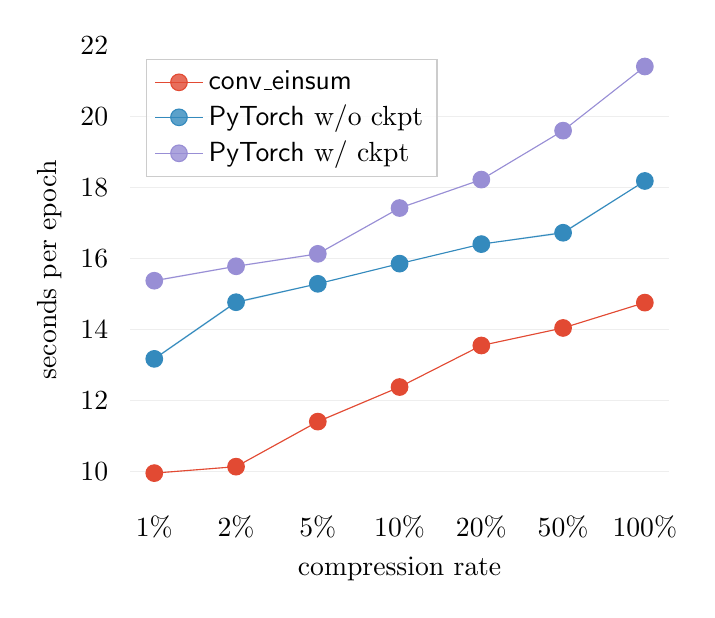
\begin{tikzpicture}

\definecolor{color0}{rgb}{0.886274509803922,0.290196078431373,0.2}
\definecolor{color1}{rgb}{0.203921568627451,0.541176470588235,0.741176470588235}
\definecolor{color2}{rgb}{0.596078431372549,0.556862745098039,0.835294117647059}

\begin{axis}[
axis line style={white},
legend cell align={left},
legend style={
  fill opacity=0.8,
  draw opacity=1,
  text opacity=1,
  at={(0.03,0.97)},
  anchor=north west,
  draw=white!80!black
},
tick align=outside,
x grid style={white},
xlabel={compression rate},
xmajorticks=true,
xtick style={draw=none},
xmin=0.7, xmax=7.3,
xtick style={color=white!33.3333333333333!black},
xtick={0,1,2,3,4,5,6,7,8},
xticklabels={,1\%,2\%,5\%,10\%,20\%,50\%,100\%,},
y grid style={white!93.3333333333333!black},
ylabel={seconds per epoch},
ymajorgrids,
ymajorticks=true,
ytick style={draw=none},
ymin=9.37454510860963, ymax=22.0011356340453,
ytick style={color=white!33.3333333333333!black}
]
\path [fill=color0, fill opacity=0.2, very thin]
(axis cs:1,9.97888939594091)
--(axis cs:1,9.94848104158397)
--(axis cs:2,10.1341301651132)
--(axis cs:3,11.3958190917175)
--(axis cs:4,12.3763176840136)
--(axis cs:5,13.5476123502911)
--(axis cs:6,14.0413649796803)
--(axis cs:7,14.7558393319893)
--(axis cs:7,14.7805985649874)
--(axis cs:7,14.7805985649874)
--(axis cs:6,14.0654411776747)
--(axis cs:5,13.5710407997148)
--(axis cs:4,12.4026890609351)
--(axis cs:3,11.4390945371537)
--(axis cs:2,10.1600878148762)
--(axis cs:1,9.97888939594091)
--cycle;

\path [fill=color1, fill opacity=0.2, very thin]
(axis cs:1,13.212937010019)
--(axis cs:1,13.1535384683386)
--(axis cs:2,14.7450545267958)
--(axis cs:3,15.2850116246708)
--(axis cs:4,15.8561679766487)
--(axis cs:5,16.4046870752762)
--(axis cs:6,16.7053913914602)
--(axis cs:7,18.177804697754)
--(axis cs:7,18.2063369673803)
--(axis cs:7,18.2063369673803)
--(axis cs:6,16.7716333181007)
--(axis cs:5,16.42428094383)
--(axis cs:4,15.8744521810938)
--(axis cs:3,15.3123507003659)
--(axis cs:2,14.8091467188384)
--(axis cs:1,13.212937010019)
--cycle;

\path [fill=color2, fill opacity=0.2, very thin]
(axis cs:1,15.4098741636846)
--(axis cs:1,15.359715998838)
--(axis cs:2,15.7725788621953)
--(axis cs:3,16.1201950872304)
--(axis cs:4,17.4164371262628)
--(axis cs:5,18.2167318277783)
--(axis cs:6,19.6044257349086)
--(axis cs:7,21.4078674336427)
--(axis cs:7,21.4271997010709)
--(axis cs:7,21.4271997010709)
--(axis cs:6,19.6170218663005)
--(axis cs:5,18.2454027336093)
--(axis cs:4,17.4457221512634)
--(axis cs:3,16.1605883847617)
--(axis cs:2,15.8085988675863)
--(axis cs:1,15.4098741636846)
--cycle;

\addplot [color0, mark=*, mark size=3, mark options={solid}]
table {%
1 9.96550999752094
2 10.1470873850588
3 11.4158439723712
4 12.3896402537851
5 13.5595994157227
6 14.0536398303251
7 14.76731840598
};
\addlegendentry{\conveinsum}
\addplot [color1, mark=*, mark size=3, mark options={solid}]
table {%
1 13.1830173239945
2 14.7788677082024
3 15.2971175402266
4 15.8651858810578
5 16.4150359613708
6 16.7352038438847
7 18.1933125245181
};
\addlegendentry{\pytorch w/o ckpt}
\addplot [color2, mark=*, mark size=3, mark options={solid}]
table {%
1 15.3839614827876
2 15.7905301555126
3 16.1408722531031
4 17.4311567858633
5 18.2321026344214
6 19.6106560296321
7 21.4176957433932
};
\addlegendentry{\pytorch w/ ckpt}
\end{axis}

\end{tikzpicture}

    }
\subcaption{RCP Train}\label{fig:imagecls-rcp-vs-pytorch-train}
\vspace{-1em}
\end{minipage}%
\hfill
\begin{minipage}[b]{.5\linewidth}
\centering
\resizebox{\textwidth}{!}{
    % This file was created by tikzplotlib v0.9.8.
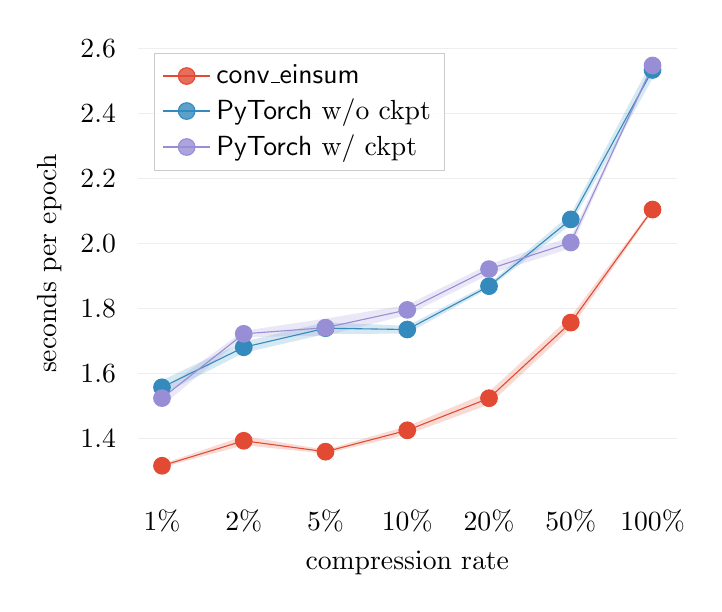
\begin{tikzpicture}

\definecolor{color0}{rgb}{0.886274509803922,0.290196078431373,0.2}
\definecolor{color1}{rgb}{0.203921568627451,0.541176470588235,0.741176470588235}
\definecolor{color2}{rgb}{0.596078431372549,0.556862745098039,0.835294117647059}

\begin{axis}[
axis line style={white},
legend cell align={left},
legend style={
  fill opacity=0.8,
  draw opacity=1,
  text opacity=1,
  at={(0.03,0.97)},
  anchor=north west,
  draw=white!80!black
},
tick align=outside,
x grid style={white},
xlabel={compression rate},
xmajorticks=true,
xtick style={draw=none},
xmin=0.7, xmax=7.3,
xtick style={color=white!33.3333333333333!black},
xtick={0,1,2,3,4,5,6,7,8},
xticklabels={,1\%,2\%,5\%,10\%,20\%,50\%,100\%,},
y grid style={white!93.3333333333333!black},
ylabel={seconds per epoch},
ymajorgrids,
ymajorticks=true,
ytick style={draw=none},
ymin=1.24857346169805, ymax=2.62702315020817,
ytick style={color=white!33.3333333333333!black},
ytick={1.2,1.4,1.6,1.8,2,2.2,2.4,2.6,2.8},
yticklabels={1.2,1.4,1.6,1.8,2.0,2.2,2.4,2.6,2.8}
]
\path [fill=color0, fill opacity=0.2, very thin]
(axis cs:1,1.32170128202879)
--(axis cs:1,1.31123026572124)
--(axis cs:2,1.37943586359388)
--(axis cs:3,1.35383196792479)
--(axis cs:4,1.4125147380759)
--(axis cs:5,1.5045691807526)
--(axis cs:6,1.73855847902859)
--(axis cs:7,2.09821307035801)
--(axis cs:7,2.11010459909695)
--(axis cs:7,2.11010459909695)
--(axis cs:6,1.77537474701384)
--(axis cs:5,1.54347203012721)
--(axis cs:4,1.43815583864567)
--(axis cs:3,1.3654502842472)
--(axis cs:2,1.40764016979432)
--(axis cs:1,1.32170128202879)
--cycle;

\path [fill=color1, fill opacity=0.2, very thin]
(axis cs:1,1.57928930643035)
--(axis cs:1,1.53615411385996)
--(axis cs:2,1.66334140504014)
--(axis cs:3,1.72147710695953)
--(axis cs:4,1.72265307494241)
--(axis cs:5,1.86189220791103)
--(axis cs:6,2.0579310830109)
--(axis cs:7,2.50675530494673)
--(axis cs:7,2.56436634618498)
--(axis cs:7,2.56436634618498)
--(axis cs:6,2.09045732611566)
--(axis cs:5,1.87629427307711)
--(axis cs:4,1.74657361604329)
--(axis cs:3,1.75756241081822)
--(axis cs:2,1.69808322827577)
--(axis cs:1,1.57928930643035)
--cycle;

\path [fill=color2, fill opacity=0.2, very thin]
(axis cs:1,1.547339830932)
--(axis cs:1,1.49956026530017)
--(axis cs:2,1.7118870869814)
--(axis cs:3,1.71640626028904)
--(axis cs:4,1.77963887616611)
--(axis cs:5,1.90444891921101)
--(axis cs:6,1.98507341910127)
--(axis cs:7,2.542796459306)
--(axis cs:7,2.55134724685929)
--(axis cs:7,2.55134724685929)
--(axis cs:6,2.02043206603775)
--(axis cs:5,1.93597701777938)
--(axis cs:4,1.81105152315929)
--(axis cs:3,1.76877109012378)
--(axis cs:2,1.73126280871942)
--(axis cs:1,1.547339830932)
--cycle;

\addplot [color0, mark=*, mark size=3, mark options={solid}]
table {%
1 1.31640031363155
2 1.39317822981615
3 1.35957493144292
4 1.42539200430426
5 1.52406284412461
6 1.75652346666184
7 2.10411776163085
};
\addlegendentry{\conveinsum}
\addplot [color1, mark=*, mark size=3, mark options={solid}]
table {%
1 1.55760821350578
2 1.68062363821
3 1.73921764819486
4 1.73527070724593
5 1.86857900731771
6 2.07382333450499
7 2.53333548435036
};
\addlegendentry{\pytorch w/o ckpt}
\addplot [color2, mark=*, mark size=3, mark options={solid}]
table {%
1 1.52429787768352
2 1.72205443814622
3 1.74087566195893
4 1.79565007027219
5 1.92109408585005
6 2.00270893324731
7 2.54707129726988
};
\addlegendentry{\pytorch w/ ckpt}
\end{axis}

\end{tikzpicture}

    }
\subcaption{RCP Test}\label{fig:imagecls-rcp-vs-pytorch-test}
\vspace{-1em}
\end{minipage}
\vspace{-1em}
\caption{\textbf{Runtime comparison between \conveinsum and \pytorch for an image classification task.} An RCP-TNN ($R=3$) is trained on the CIFAR-10 dataset. Runtimes are averaged over 3 random runs, and error bars are denoted by the shaded areas.}\label{fig:imagecls-rcp-vs-pytorch}
\vspace{-1em}
\end{figure}

\end{document}